\documentclass{beamer}

\usepackage{subfigure}
\usepackage{graphicx}
\usepackage{sidecap}
\usepackage{caption}
%\usepackage{subcaption}
\captionsetup{compatibility=false}
\usepackage{appendixnumberbeamer}
\usepackage{amsmath}
% --
\usepackage{multirow}
\usepackage{xcolor}
\usepackage{setspace}
\usepackage{hyperref}
\usepackage{anyfontsize}

\beamertemplatenavigationsymbolsempty
\setbeamertemplate{footline}

\newenvironment{itemise} {\begin{itemize} \setlength{\itemsep}{0.2cm}} {\end{itemize}}
\usepackage[labelformat=empty]{caption}
\setbeamertemplate{sections/subsections in toc}[square]

%% COLORS
\definecolor{Gray}{gray}{0.9}
\definecolor{dblue}{rgb}{0.132,0.1,0.27}
\definecolor{mint}{cmyk}{1.0, 0.2, 0.6, 0.05}
\definecolor{ant}{cmyk}{0.5, 0.1, 0.0, 0.45}
\definecolor{lgray}{cmyk}{0.12, 0.0, 0.0, 0.17}
\definecolor{lred}{cmyk}{0.0, 0.9, 0.7, 0.0}


\usepackage{etoolbox}% http://ctan.org/pkg/etoolbox 
\usepackage{booktabs}

\newenvironment{literatur}{%
  \parskip2pt \parindent0pt \raggedright
  \def\lititem{\hangindent=0.5cm \hangafter1}}{%
  \par\ignorespaces}

\newcommand{\tb}[1]{{\color{blue}{\textbf{#1}}}}
\newcommand{\tm}[1]{{\color{mint}{\textbf{#1}}}}
\newcommand{\tr}[1]{{\color{red}{\textbf{#1}}}}
% Ilya: packages

\usepackage{tikz}
\usepackage{lmodern}
\usepackage{enumitem}

% Ilya: my commands

\newenvironment{mytemize}
{\vfill\itemize[nolistsep,itemsep=\fill,label=\color{blue}{$\triangleright$}]}
  {\enditemize}
\newenvironment{mynumerate}
{\vfill\enumerate[nolistsep,itemsep=\fill,label=\arabic*.]}
  {\endenumerate}

\newcommand{\hitem}[1]{
  {\color{blue}{$\triangleright$}} 
  {#1} 
  {\hfill}
}

\setlist[itemize]{label= \color{blue}{$\triangleright$}}

\newcommand{\rarr}{$\Rightarrow$\ }

\AtBeginSection{%
\ifshowtoc
\begin{frame}
    \tableofcontents[currentsection, subsectionstyle=show/show/hide]
\end{frame}
\fi
}

%\href{<Ziel>}{<Eingefasster Text>} 

%\logo{\includegraphics[height=0.7cm]{BdFlogo.eps}\hspace{300pt}\vspace{-5pt}}
%\logo{\includegraphics[height=0.8cm]{BdFlogo.eps}}
%\logo{\pgfputat{\pgfxy(-6.2,-0.5)}{\pgfbox[center,base]{\includegraphics[height=0.8cm]{BdFlogo.eps}}}}

%------------------------------------------------------------------------------------
% TITLE
%------------------------------------------------------------------------------------
\title[PSME]{Macroeconomics\\ Lecture 1 -- Introduction \& IS-TR }
\author[I. Eryzhenskiy]{Ilya Eryzhenskiy}
\institute[BdF]{PSME Panth\'{e}on-Sorbonne Master in Economics}
\date[PSME macro]{Fall 2022}

%---BEGIN------------------------------------------------------------------------------
\begin{document}
%---BEGIN------------------------------------------------------------------------------
\begin{frame}
\maketitle
\end{frame}

%---FRAME------------------------------------------------------------------------------
\section{What is Macro? Why Macro?}

\begin{frame}{%
\protect\hypertarget{macroeconomics-object-of-study}{%
Macroeconomics: objects}}

Main objects of study --- \emph{aggregate} measures of economic activity.
\vfill
Interactions of various \textbf{markets}\ldots{}
\vfill
\begin{columns}[c]
  \column{0.48\textwidth} 
  \begin{mytemize}
\item
  Goods:

  \begin{mytemize}
  \item
    Consumption goods
  \item
    Investment goods (capital)
  \end{mytemize}
\item
  Services
  \end{mytemize}
  \column{0.48\textwidth} 
\begin{mytemize}
 
\item
  Labor
\item
  Finance:

  \begin{mytemize}
   
  \item
    Banking
  \item
    Market finance
  \end{mytemize}
\item
  Currency
\end{mytemize}

\end{columns}
\vfill
\ldots{}and \textbf{policies}: 
\vfill
\ 
\hitem{Monetary}
\hitem{Fiscal}
\hitem{Regulation}
\\
\vfill
One (even huge) market is not ''macro`` enough: e.g. real estate

\end{frame}

\begin{frame}{Macroeconomics: motivation}

  Why care for the macro-economy?
  \vfill
\begin{mytemize}
\item As \tb{households}, we are all affected: 
  \begin{mytemize}
  \item Crises \rarr unemployment: lives depend on business cycles
  \item Need to check macro for big decisions: housing, retirement, own business\ldots
  \end{mytemize}
\item \tb{Businesses}: cycles influence demand and supply chains, interest rates, exchange rates, inflation\ldots
\item \tb{Policymakers}: macro policy is influential. In addition macro phenomena (over-)associate with politics \rarr accountability of politicians
\end{mytemize}
\end{frame}

\begin{frame}{%
\protect\hypertarget{macroeconomics-rules-keynes}{%
Macroeconomics rules: Keynes}}

\begin{quote}
Practical men who believe themselves to be quite exempt from any
intellectual influence, are usually the slaves of some defunct
economist.
\end{quote}

\begin{flushright}
John Maynard Keynes
\end{flushright}

\vfill
\textit{N. B.}: Keynes \tr{is} the most influential macroeconomist to date\ldots
\end{frame}
%---FRAME------------------------------------------------------------------------------

%---FRAME------------------------------------------------------------------------------
%---FRAME------------------------------------------------------------------------------
\begin{frame}{Methodology of Macroeconomics: Theory}

\begin{mytemize}
\item Macro deals with complex relationships of dynamic variables
\item Theory with a good deal of \textit{abstraction} necessary:
\begin{mytemize}
\item \tb{exogenous} variables are taken as given, ``out of nowhere''
    \begin{mytemize}
        \item their changes often called \tr{shocks}
    \end{mytemize}
\item \tb{endogenous} variables are explained by the model
\end{mytemize}
\end{mytemize}

\begin{center}
\begin{figure}[h!]
	\subfigure{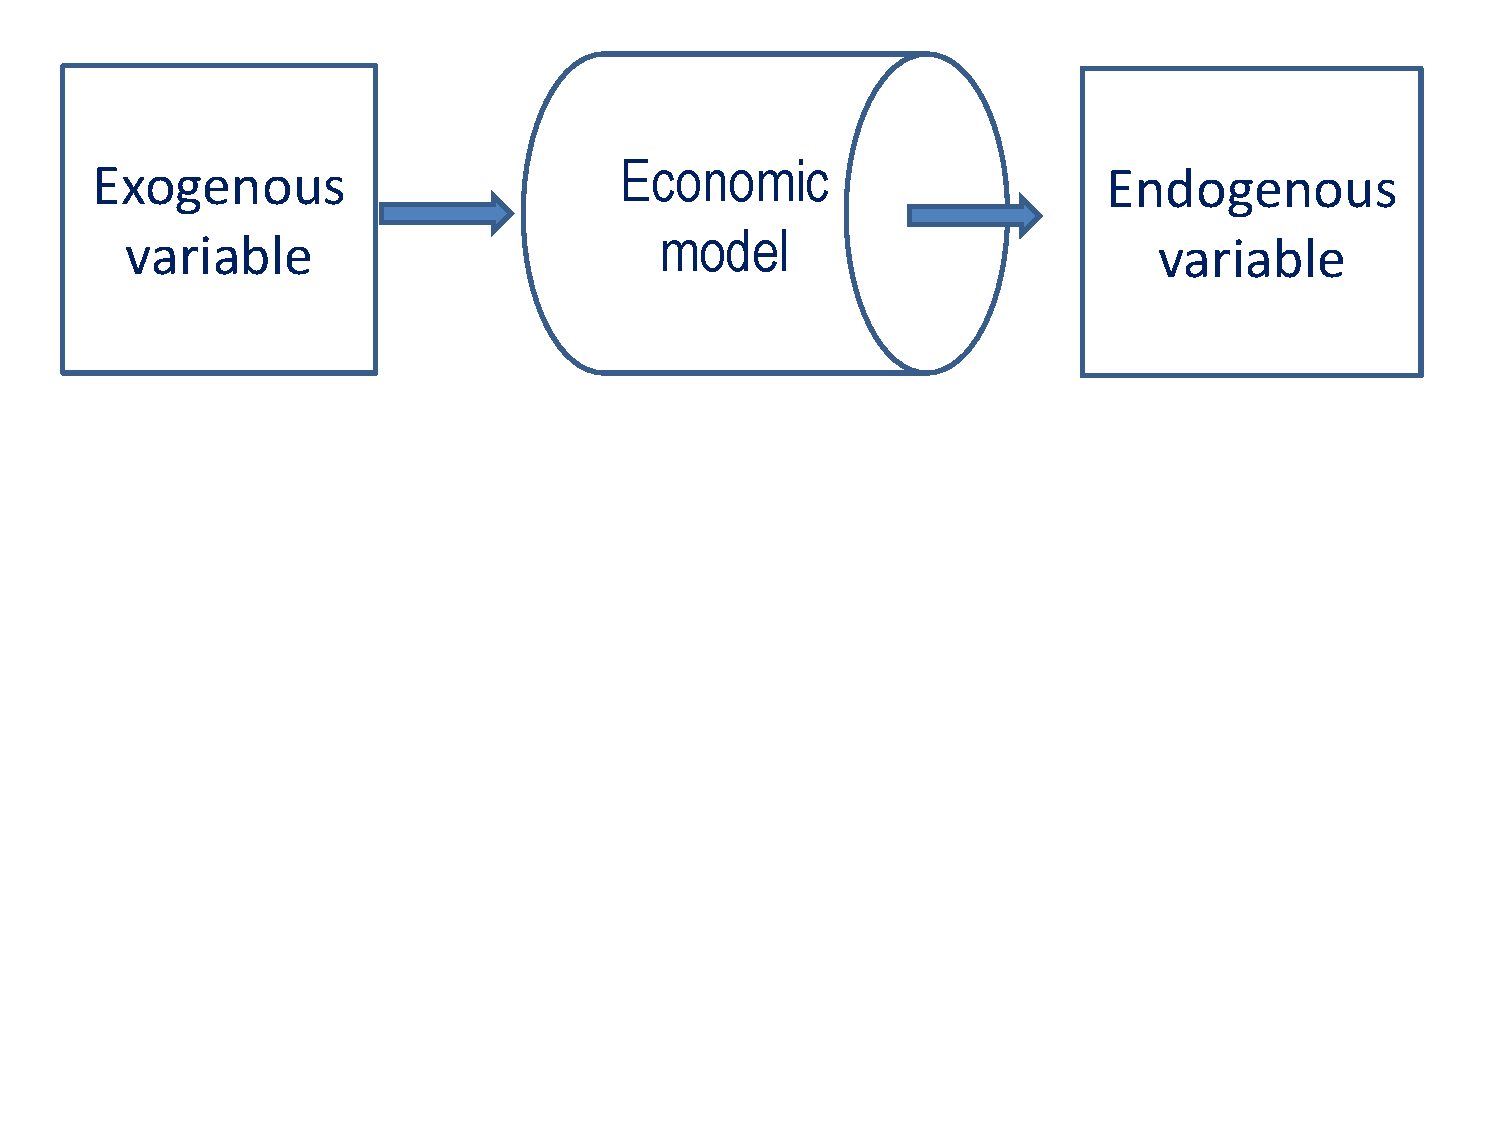
\includegraphics[trim=0 300 0 0,clip,width=0.7\textwidth]{FIGURES/1_EconModel}
	}      
	%[trim=left bottom right top
%	\label{fig:GPD} 
\end{figure}
%\vspace{-2mm}
%\begin{minipage}{0.9\columnwidth}
%\tiny	
%\textbf{Note.} .\\
% \textbf{Source.} Jorda-Schularick-Taylor Macrohistory Database \href{http://www.macrohistory.net/data/}{[Link]} .\\
%\end{minipage}
\end{center}

\end{frame}
%% baby background:
%{
%\usebackgroundtemplate%
%{%
%  %\begin{figure}[b!]
%  \begin{tikzpicture}
%	\draw node[opacity=0] at (15,6) {
\includegraphics[width=0.3\paperwidth]{baby_logo.png}};%
%    \draw node[opacity=0.3] at (14.5,-0.4) {
\includegraphics[width=0.3\paperwidth]{baby_logo.png}};%
%    %\draw node[opacity=0.8] at (15.3,6) {\includegraphics[width=0.23\paperwidth]{../PSE_logo.png}};%
%	\draw node[opacity=0] at (10.3,-1.4) {
\includegraphics[width=0.37\paperwidth]{baby_logo.png}};%
%	\draw node[opacity=0] at (6,-1.4) {
\includegraphics[width=0.3\paperwidth]{baby_logo.png}};%
%  \end{tikzpicture}
%  %\end{figure}
%}
%\begin{frame}{Models can be fun}
%   Macroeconomic crises and monetary policy can be seen on a real-life historical example of\ldots a \tb{baby-sitters cooperative} 
%\vfill
%  \begin{itemize}
%	\item Parents babysit each others' children
%	  \vfill
%	\item A currency --- \textit{scrpis} --- introduced to promote fairness
%	  \vfill
%	  \begin{itemize}
%		\item 1 \textit{scrip} $=$ 1 hour of baby-sitting
%	  \vfill
%	\item rigid price set \textit{exogenously}, rather than \textit{endogenously} determined by market
%	  \vfill
%	\item each family receives a number of scrips to begin with
%	  \vfill
%	  \end{itemize}
%	  \vfill
%		\item if a couple wants more babysitting for their child, need to babysit more
%	  \vfill
%	\item some have busy periods: cannot babysit, but need babysitting $\Rightarrow$ need excess \textit{reserves} of scrips
%  \end{itemize}
%  Source: Joan and Richard Sweeney ``Monetary Theory and the Great Capitol Hill Baby-Sitting Co-op Crisis.'' Journal of Monetary Economics, 1978.
%\end{frame}
%\begin{frame}{A crisis}
%  \begin{itemize}
%	\item Some babysitting-scripts accounting problems $\Rightarrow$ an episode with a decrease of scrips in circulation: an \tr{exogenous shock} 
%	  \vfill
%	\item parents worried they don't have enough reserve scrips and reduce spending\ldots 
%	  \vfill
%	\item \ldots others have less scrips, worried they don't have enough, and so on
%	  \vfill
%	  \begin{itemize}
%		\item A vicious cycle / \textit{coordination failure} / bad \textit{equilibrium}
%	  \end{itemize}
%	  \vfill
%	\item a monetary problem (exogenous) causing a decline of activity (endogenous): babysitting has stopped
%  \end{itemize}
%\end{frame}
%}
%---FRAME------------------------------------------------------------------------------
\begin{frame}{Methodology of Macroeconomics: Data}


\begin{mytemize}
\item Unrealistic models are fine as long they:
  \begin{mytemize}
	\item give novel insights (M. Friedman)
	\item are \textit{falsifiable} i.e. can be proven wrong (K. Popper)
  \end{mytemize}
\item Confronting macro theories with data is challenging:
\begin{mytemize}
\item aggregate indices: measurement problems
\item correlation vs. causality: experimental approach, as in applied micro, rarely applicable
\item 
tb{expectations} are crucial, but never directly measurable
\end{mytemize}
\item Solutions:
\begin{mytemize}
\item vector autoregression (VAR) approach (Nobel prize of C. Sims) -- estimate \tb{impulse responses} to shocks with (almost) no model
\item estimate theoretical models, compare outputs to data

\end{mytemize}
\end{mytemize}

\end{frame}

{
\usebackgroundtemplate%
{%
  %\begin{figure}[b!]
  \begin{tikzpicture}
	\draw node[opacity=0] at (15,6) {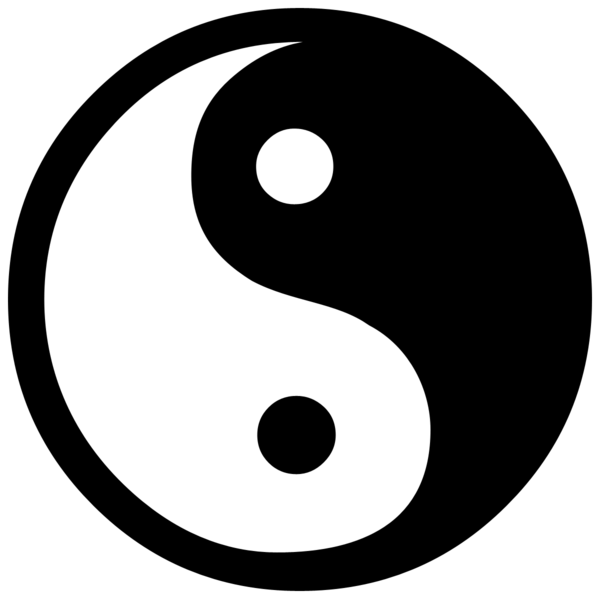
\includegraphics[width=0.3\paperwidth]{FIGURES/yin_yang.png}};%
    \draw node[opacity=0.05] at (14.5,-0.4) {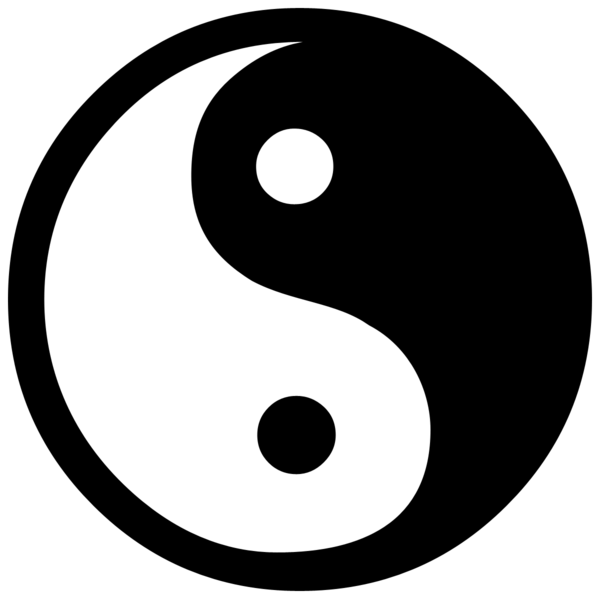
\includegraphics[width=0.3\paperwidth]{FIGURES/yin_yang.png}};%
    %\draw node[opacity=0.8] at (15.3,6) {\includegraphics[width=0.23\paperwidth]{../PSE_logo.png}};%
	\draw node[opacity=0] at (10.3,-1.4) {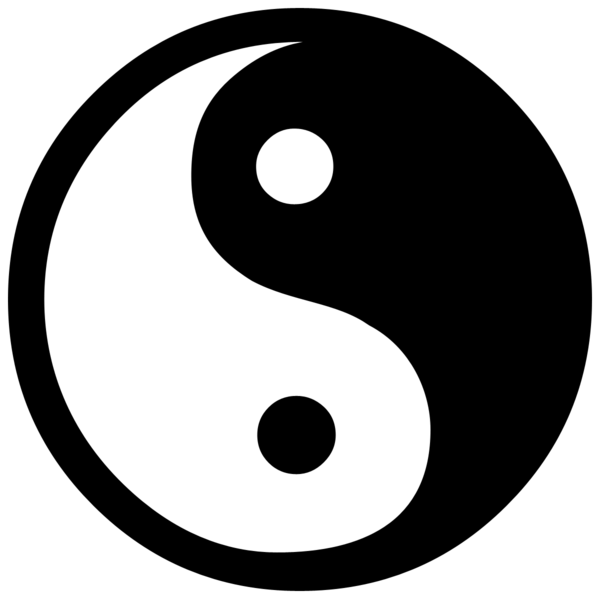
\includegraphics[width=0.37\paperwidth]{FIGURES/yin_yang.png}};%
	\draw node[opacity=0] at (6,-1.4) {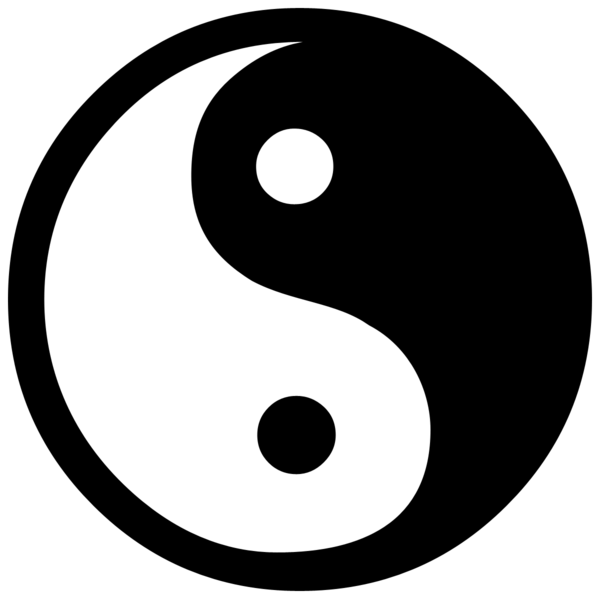
\includegraphics[width=0.3\paperwidth]{FIGURES/yin_yang.png}};%
  \end{tikzpicture}
  %\end{figure}
}
\begin{frame}{Macro dichotomies}
  		\begin{center}
		  \underline{\textbf{Macroeconomics}}\\
				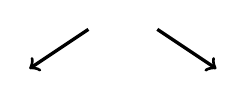
\begin{tikzpicture}[xscale = .5, yscale = .5]
				  \draw[->, very thick] (-0.5, 1)--(-2, 0) ;
		\draw[->, very thick] (1.25, 1)--(2.75, 0) ;
		\end{tikzpicture}
		\end{center}
		\begin{columns}[T]
				\column{.48\textwidth}
				\centering
			  \underline{\textbf{Theoretical}}
				\begin{itemize}
				  \item A zoo of models (see next slides)
				  \item \tb{Focus for this course}
				\end{itemize}
\column{.48\textwidth} 
				\centering
\underline{\textbf{Empirical}}
				\begin{itemize}
					\item Model estimation
					  \begin{itemize}
						  \item 
							introduction with practical implementation (coding) \tr{in TD}
						\end{itemize}
				  \item Time series \& VAR econometrics 
					\begin{itemize}
						\item Econometrics class (?)
					  \end{itemize}
				\end{itemize}
				\end{columns}
		\vfill
\end{frame}


\begin{frame}{Macro dichotomies}
  		\begin{center}
		  \underline{\textbf{Macroeconomic models}}\\
				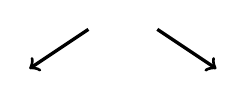
\begin{tikzpicture}[xscale = .5, yscale = .5]
				  \draw[->, very thick] (-0.5, 1)--(-2, 0) ;
		\draw[->, very thick] (1.25, 1)--(2.75, 0) ;
		\end{tikzpicture}
		\end{center}
		\begin{columns}[T]
				\column{.48\textwidth}
				\centering
			  \underline{\textbf{Short-run}}
				\begin{itemize}
				  \item Most of macroeconomists' job. Why?
					\begin{itemize}
					  \item Immediately applicable?
					  \item Most politicians' focus?
					\end{itemize}
				  \item \tb{Focus of this course}
				\end{itemize}
\column{.48\textwidth} 
				\centering
\underline{\textbf{Long-run}}
				\begin{itemize}
				  \item More substantial problems
				  \item See Growth course (unless you are in financial track!)
				\end{itemize}
				\end{columns}
		\vfill
\end{frame}
\begin{frame}{Macro dichotomies}
  		\begin{center}
		  \underline{\textbf{Macroeconomic models}}\\
				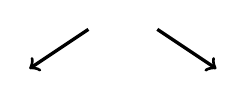
\begin{tikzpicture}[xscale = .5, yscale = .5]
				  \draw[->, very thick] (-0.5, 1)--(-2, 0) ;
		\draw[->, very thick] (1.25, 1)--(2.75, 0) ;
		\end{tikzpicture}
		\end{center}
		\begin{columns}[T]
				\column{.48\textwidth}
				\centering
			  \underline{\textbf{Dynamic}}
				\begin{itemize}
				  \item The modern approach
				  \item[] \tb{Most of the course}
				\end{itemize}
\column{.48\textwidth} 
				\centering
\underline{\textbf{Static}}
				\begin{itemize}
				  \item Keynes-Hicks heritage (20th century)
				  \item[] \tr{Beginning of course} 
				\end{itemize}
				\end{columns}
		\vfill
\end{frame}

\begin{frame}{Macro dichotomies}
  		\begin{center}
		  \underline{\textbf{Macroeconomic models}}\\
				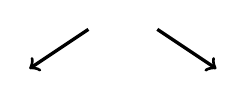
\begin{tikzpicture}[xscale = .5, yscale = .5]
				  \draw[->, very thick] (-0.5, 1)--(-2, 0) ;
		\draw[->, very thick] (1.25, 1)--(2.75, 0) ;
		\end{tikzpicture}
		\end{center}
		\begin{columns}[T]
				\column{.48\textwidth}
				\centering
			  \underline{\textbf{Closed economy}}
				\begin{itemize}
				  \item Wild simplification, but\dots
				  \item \dots most macro scholars based in the U.S. --- large and independent enough \rarr closed economy is 
					most studied model
				  \item[] \tb{around $70$\% of course} \end{itemize}
\column{.48\textwidth} 
				\centering
\underline{\textbf{Open economy}}
				\begin{itemize}
				  \item Small open economy models: country as \textit{price-taker} 
      \item[] \tr{around $30 \%$ of course}
				  \item Large open economy models: country influences prices \item[] \tr{rarely discussed in course}
				  %\item Open economy parts of course are mostly about \tr{small open economy} 
				\end{itemize}
				\end{columns}
		\vfill
\end{frame}

\begin{frame}{Macro dichotomies}
  		\begin{center}
		  \underline{\textbf{Macroeconomic models}}\\
				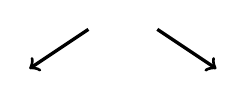
\begin{tikzpicture}[xscale = .5, yscale = .5]
				  \draw[->, very thick] (-0.5, 1)--(-2, 0) ;
		\draw[->, very thick] (1.25, 1)--(2.75, 0) ;
		\end{tikzpicture}
		\end{center}
		\begin{columns}[T]
				\column{.48\textwidth}
				\centering
				\underline{\textbf{Flexible price (neoclassical)}}
				\begin{itemize}
				  \item Usually result in optimal allocations
					\begin{itemize}
					  \item \textit{laissez-faire} economics
					  \end{itemize}
					  \item Useful to understand how a perfect world would work --- normative approach
				  \item[] \tb{Most of the course}
				\end{itemize}
\column{.48\textwidth} 
				\centering
				\underline{\textbf{Sticky price (Keynesian)}}
				\begin{itemize}
				  \item Associated with corrective interventions, such as Keynesian demand management
				  \item[] \tr{Beginning}, then \tr{second half} of course
				\end{itemize}
				\end{columns}
		\vfill
\end{frame}

 
}

\section{Old Keynesian macro: IS-TR}


%---FRAME------------------------------------------------------------------------------

%---FRAME------------------------------------------------------------------------------
\subsection{The Goods Market}
%---FRAME------------------------------------------------------------------------------
\begin{frame}{Price rigidity}

Central \tb{Keynesian assumption:} Prices do not adjust immediately \\

\begin{mytemize}
\item Price rigidity associated with time horizon: 
  \begin{mytemize}
	  \item very short term --- fixed prices (extreme case)
	  \item short term --- sticky (slow moving) prices 
		\item medium or long term --- flexible prices
	\end{mytemize}
\item If demand is insufficient under current (fixed) prices \rarr \tb{demand-driven equilibrium}. \textcolor{mint}{Why? Recall micro equilibrium diagram}
\begin{mytemize}
    \item Keynes' context was the Great Depression \rarr natural to assume insufficient demand. Later, this assumption became an axiom for Keynesians
\end{mytemize}

\end{itemize}

\end{frame}
%---FRAME------------------------------------------------------------------------------

%\begin{frame}{Price rigidities: data}
%
%\begin{itemize}
%\small
%\item Evidence from the euro area points to sticky prices
%\end{itemize}
%
%\begin{center}
%%{\small
%%Figure. Liability = a promise to payout the holder of the note  \\
%%}
%
%%\vspace{-2mm}
%\begin{figure}[h!]
%%\caption{Figure. Capital share US, 1946-2018
%	%\subfigure{\includegraphics<1>[trim=80 60 100 70,clip,width=0.75\textwidth]{FIGURES/3_Autarky}
%	%}
%	\subfigure{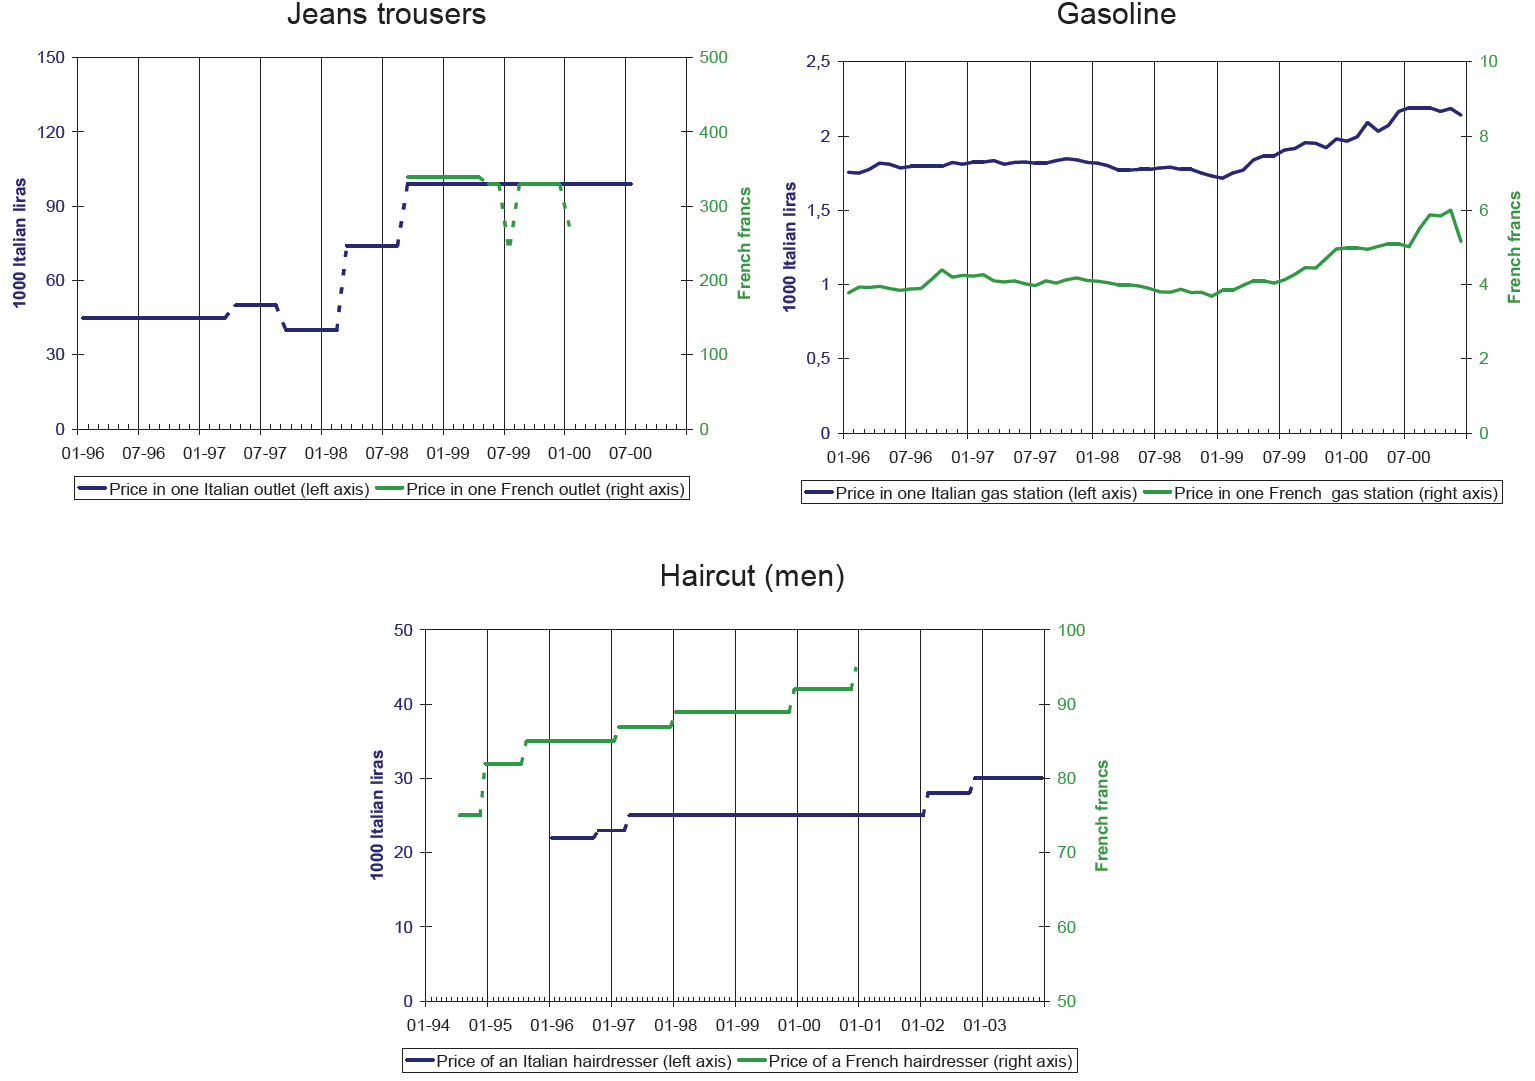
\includegraphics[trim=0 0 0 0,clip,width=0.8\textwidth]{FIGURES/6_PriceChangesEA}
%	}      
%	%\subfigure{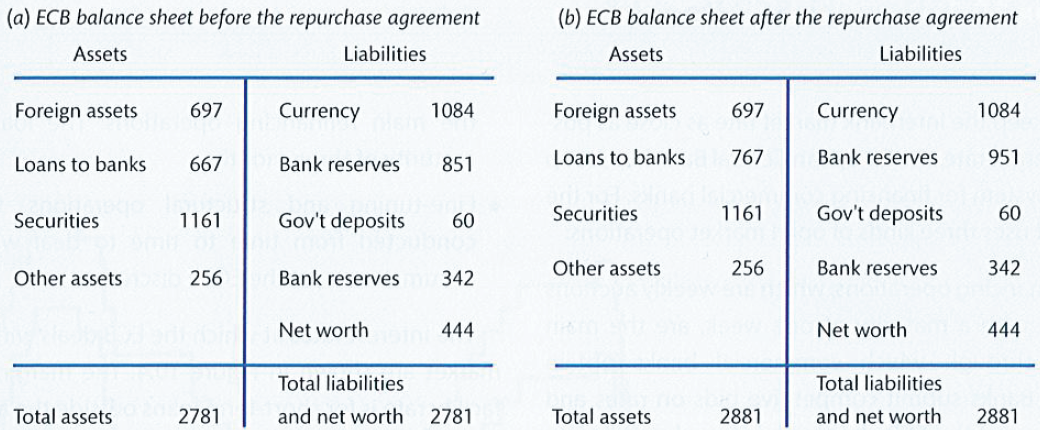
\includegraphics[trim=0 00 0 00,clip,width=0.6\textwidth]{FIGURES/5_CB_balance_sheet_OMO}
%	%} 
%	
%%	\label{fig:GPD} 
%	%[trim=left bottom right top
%\end{figure}
%%\vspace{-2mm}
%
%\begin{minipage}{1.0\columnwidth}
%\tiny	
%\textbf{Note.} Actual examples of trajectories, extracted from the French and Italian CPI databases. The dotted lines indicate events of price changes.
%\textbf{Source.} Dhyne et al (2005) 'Price setting in the euro area: Some stylized facts from individual consumer price data', Figure 1.\\
%\end{minipage}
%\end{center}
%
%\end{frame}

%\begin{frame}{Preview: General equilibrium}
%
%\begin{itemize}
%\small
%\item Focus: \tb{goods market} \& \tb{money market}
%\item \tm{General equilibrium}: all markets clear simultaneously
%\item $\rightarrow$ market conditions are mutually consistent
%%\item Preview: Figure
%\begin{itemize}
%\small
%\item (\emph{Note:} We mostly exclude the foreign exchange market in this lecture.)
%\end{itemize}
%\end{itemize}
%
%\begin{center}
%%{\small
%%\tb{Figure.} Frequency of price increases and price decreases \\
%%}
%
%%\vspace{-2mm}
%\begin{figure}[h!]
%%\caption{Figure. Capital share US, 1946-2018
%	%\subfigure{\includegraphics<1>[trim=80 60 100 70,clip,width=0.75\textwidth]{FIGURES/3_Autarky}
%	%}
%	\subfigure{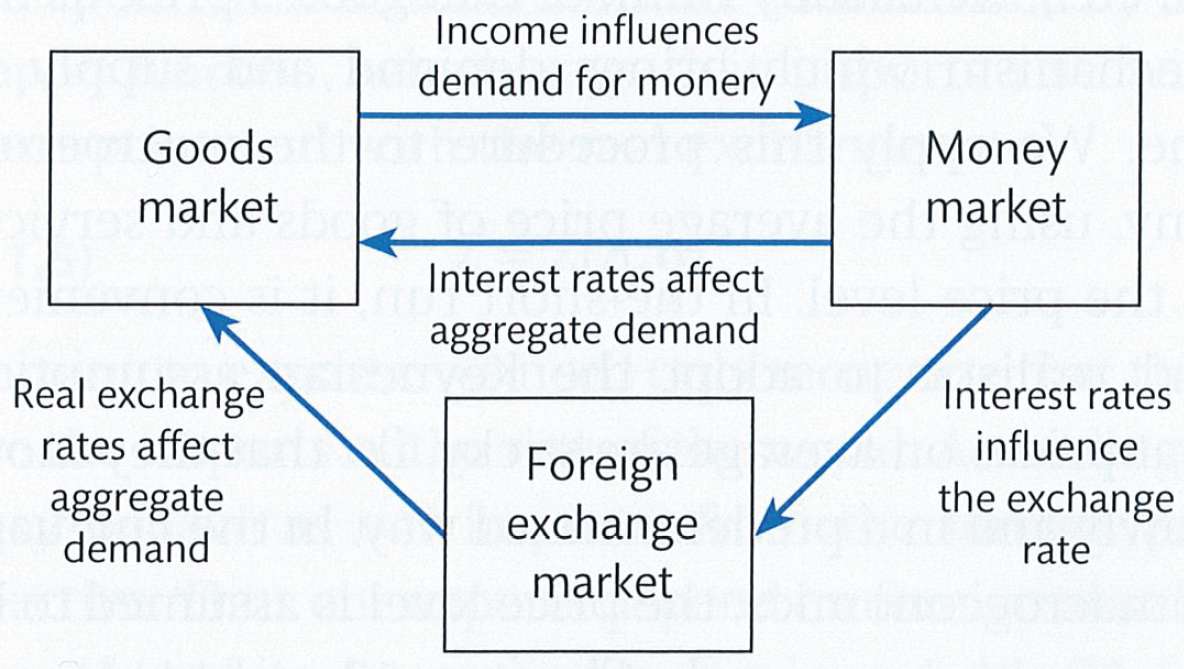
\includegraphics[trim=0 0 0 0,clip,width=0.75\textwidth]{FIGURES/6_GE}
%	}      
%	%\subfigure{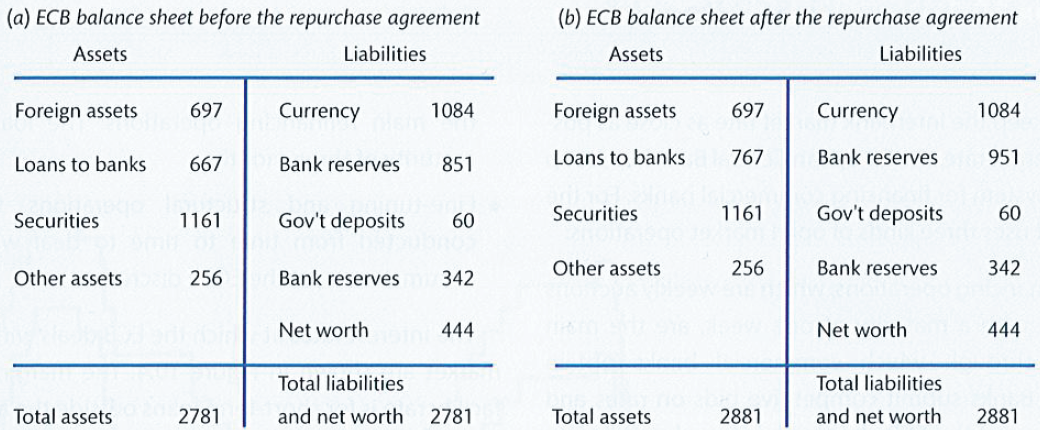
\includegraphics[trim=0 00 0 00,clip,width=0.6\textwidth]{FIGURES/5_CB_balance_sheet_OMO}
%	%} 
%	
%%	\label{fig:GPD} 
%	%[trim=left bottom right top
%\end{figure}
%%\vspace{-2mm}
%
%\begin{minipage}{0.6\columnwidth}
%\tiny	
%%\textbf{Note.} Actual examples of trajectories, extracted from the French and Italian CPI databases. The dotted lines indicate events of price changes.
%\textbf{Source.} Burda and Wyplosz (2017), Figure 11.2.\\
%\end{minipage}
%\end{center}
%
%
%\end{frame}
%---FRAME------------------------------------------------------------------------------
\begin{frame}{Desired demand for goods -- closed economy}
Assume a single good is used for consumption 
($C$), investment ($I$) and government consumption/ investment ($G$). \\
Desired demand of the three sectors: $C+I+G$ \\
Denote $Y$ the supply of goods:
\begin{align*}
\underbrace{Y}_{\text{supply of goods}}=\underbrace{C+I+G}_{\text{desired demand}}
\end{align*}
same formula as GDP decomposition in national accounts, \textbf{but}:
\begin{mytemize}
\item It is a statement about a \tb{demand driven equilibrium}: supply adjusts to demand
\item OK, but what happens if demand suddenly changes?
\begin{itemize}
\item classical price adjustment does not work (\tb{fixed prices} assumption)
\item instead, firms accumulate and decumulate \tb{inventories} 
\end{itemize}
\end{mytemize}
\end{frame}

\begin{frame}{Desired demand for goods -- open economy}
Supply and demand must be adjusted for exports and imports:
\begin{align*}
Y + \underbrace{Im}_{\text{Imports}} &= C + I + G + \underbrace{Ex}_{\text{Exports}} \\
\text{or, using\ \ } TB &= Ex - Im, \\
Y &=C+I+G+\underbrace{TB}_{\text{trade balance}} \end{align*} 

\begin{mytemize}
    \item Desired demand includes \tb{trade balance (TB)}
    \begin{mytemize}
    \item TB also known as net exports or \tb{primary current account (PCA)}
        \item \textcolor{mint}{Notation:} PCA is used instead of TB in BW textbook
        %\item We will define what is current account in 3 lectures
    \end{mytemize}
\end{mytemize}
\end{frame}
%---FRAME------------------------------------------------------------------------------
\begin{frame}{Consumption function}

\begin{equation*}
C= C(\underbrace{Y-T}_{+}, \underset{+}{\Omega}) 
\end{equation*}
\begin{mytemize}
\item $Y$ is household income (since GDP is sum of incomes) 
\item $T$ is tax (assumed lump-sum, i.e.~independent of any household characteristics)
\item[\rarr] $Y-T$ is \tb{disposable income} 
\item $\Omega$ is wealth
\end{mytemize}
\vspace{1cm}

How to measure the reaction of consumption to a change in disposable income? \\ Take a derivative: $$mpc = \frac{\partial C}{\partial (Y-T)}$ is the \tb{marginal propensity to consume}. Assumption $0<mpc< 1$ central to Keynesian analysis
\end{frame}

\begin{frame}{Investment function}
\begin{equation*}
I = I(\underset{+}{q},\underset{-}{r}) 
\end{equation*}
Tobin's $q$ is the ratio of \tb{market value of installed capital} and \tb{replacement cost of capital}%$\left( q=\frac{\textnormal{market value of installed capital}}{\textnormal{replacement cost of capital}}\right)$
    \begin{itemize}
        \item \textcolor{mint}{For now, think of ``investor sentiment'' that encourages investment. We will formalize Tobin's $q$ in the RBC model}
    \end{itemize}
    \vfill
Real interest rate $r$ is defined as: \begin{equation*}
    r = \underbrace{i}_{\text{nominal interest}} - \underbrace{\pi^e}_{\text{expected inflation}}
\end{equation*}

\textbf{A rise in the real interest discourages investment}: borrowing becomes more expensive, future incomes are valued less ($r$ is used in \tb{discounting})
\end{frame}

\begin{frame}{Trade balance function}
    \tb{Trade balance function}
    $$
TB = Ex(\underset{+}{Y^*},\underset{-}{\sigma}) \textcolor{red}{-} Im(\textcolor{red}{\underset{+}{Y}},\underset{+}{\sigma})= TB(\textcolor{red}{\underset{-}{Y}}, \underset{+}{Y^*},\underset{-}{\sigma}) 
$$

\begin{mytemize}
\item $Y^*$ is output/incomes of rest of the world 
    \item $Y^*$ as argument of $Ex(\cdot)$ and $Y$ as argument of $Im(\cdot)$ are shortcuts: all determinants of foreign demand $C^*+I^*+G^*$ might be relevant for $Ex$ and all local demand might be relevant for $Im$
    \item $\sigma$ is \tb{real exchange rate}: how expensive are domestic goods relative to foreign goods \tm{(more on this next week)}
\end{mytemize}

\end{frame}
%---FRAME------------------------------------------------------------------------------
%\begin{frame}{Aggregate demand}
%
%\tb{Import function}
%\begin{equation}
%Z = Z(\underset{+}{A},\underset{+}{\sigma}) \tag{11.5}
%\end{equation}
%\begin{itemize}
%\small
%\item domestic absorption, $A=C+I+G$
%\item real exchange rate (\emph{appreciation}), ($\sigma=SP/P^*$, with $S$ denoting the nominal exchange rate, and $P^*$ the foreign price level)
%\end{itemize}
%
%\tb{Export function}
%\begin{equation}
%X = X(\underset{+}{A^*},\underset{-}{\sigma}) \tag{11.6}
%\end{equation}
%\begin{itemize}
%\small
%\item foreign absorption, $(A^*)$
%\item real exchange rate (\emph{depreciation}), ($\sigma$)
%\end{itemize}
%
%\tb{Net exports}
%\begin{align}
%NX = &X(\underset{+}{A^*},\underset{-}{\sigma})-Z(\underset{+}{A},\underset{+}{\sigma}) \nonumber\\
% =	 & NX(\underset{-}{A},\underset{+}{A^*},\underset{-}{\sigma})   \nonumber\\
%\text{simplification} \Leftrightarrow NX = & NX(\underset{-}{Y},\underset{+}{Y^*},\underset{-}{\sigma})	\tag{11.8}
%\end{align}
%
%\end{frame}
%---FRAME------------------------------------------------------------------------------
\begin{frame}{Desired demand (DD) function}

\begin{align*}
DD &= C(\underset{+}{Y-T}, \underset{+}{\Omega}) + I(\underset{+}{q},\underset{-}{r}) + TB(\underset{-}{Y}, \underset{+}{Y^*},\underset{-}{\sigma})+ G \\
&= DD(Y,r, \dots)
\end{align*}

where ``$\dots$'' regroups exogenous variables: $T, G, \Omega, q, Y^*, \sigma$.
\\ \vfill
What is the influence of $Y$
 on DD? Depends on two derivatives: $\frac{\partial C}{\partial Y} = \frac{\partial C}{\partial (Y-T)} (= mpc)$ and $\frac{\partial TB}{\partial Y} (= -\frac{\partial Im}{\partial Y})$, which is the negative of \tb{marginal propensity to import (mpm)}. \\
 \vfill
 Assume reaction of domestic consumption to income is stronger than reaction of imports. \\ 
 \vfill
 Then, DD increases in domestic income, with derivative $\frac{\partial C}{\partial Y} - \frac{\partial Im}{\partial Y} = mpc - mpm$, assumed positive, but \textbf{below 1} \textcolor{mint}{(why?)}
\end{frame}
%---FRAME------------------------------------------------------------------------------
\begin{frame}{Goods market equilibrium: comparative statics}

Equilibrium condition can be written as $Y = DD(Y, r, \dots)$. \\
Assume an increase in $DD$ by 1 unit, e.g. because of $G$:
\begin{mytemize}
\item $Y$ must increase in response by the same amount. Is $Y = DD(Y, r, \dots)$ verified? No, because DD increases again: 
\begin{mytemize}
\small
\item $C\uparrow$, $TB\downarrow$
\item The effect on $C$ dominates
\item $DD$ increases by $mpc - mpm$
\end{mytemize}
\item $Y$ rises by $mpc - mpm$ in response
\item the cycle repeats until equilibrium restored
\end{mytemize}
The model is not dynamic, so the adjustment assumed to happen immediately. What is the ultimate increase in $Y$? \\ \vfill Answer:  $1/(1-mpc+mpm)$ -- a sum of geometric series with coefficient $mpc-mpm$. 
\end{frame}

\begin{frame}{The Keynesian Multiplier}
   The ratio of increase in GDP and the increase of government spending is called the \tb{Keynesian multiplier} of government spending. \\
   \vfill
   For small changes (shocks) of government spending $d G$, the increase in GDP is $\frac{1}{1-mpc+mpm} d G$. The multiplier is then $$\frac{d Y}{d G} = \frac{1}{1-mpc+mpm}$$ so it is a derivative of \textbf{equilibrium} GDP with respect to government expenditure. \\
   \vfill
   The multiplier is the same for large shocks if the model is linear \textcolor{mint}{this will be seen in TD} 
\end{frame}

\begin{frame}{Goods market equilibrium: the 45$^{\circ}$ diagram}
    
\end{frame}
%---FRAME------------------------------------------------------------------------------
%\begin{frame}{Goods market equilibrium}{Example 2: Keynesian multiplier}
%
%Consider: \tb{Increase in public pending, $\Delta G$}
%\begin{itemize}
%\small
%\item $DD\uparrow$, firms will produce more, ..., $Y\uparrow$
%\item \tm{"Multiplier"}: \emph{By how much does output change, $\Delta Y$?}
%\begin{itemize}
%\small
%\item firms will increase production by $\Delta G$
%\item this generates new income, thus $C\uparrow$ ($I$ too, if $Y\uparrow$\rarr$q\uparrow$)%, $NX\downarrow$
%\item[$\rightarrow$] $Y\uparrow, C\uparrow, Y\uparrow$
%\item additional spending $\Delta C$ is smaller due to \textit{leakages}, so $\Delta Y_2< \Delta Y_1$
%\item leakages (closed economy): \emph{savings, taxes (if proportional)}
%\begin{itemize}
%\small
%\item \tb{marginal propensity to consume}, $0<c<1$
%%\item \tb{marginal propensity to import}, $0<z<1$
%\end{itemize}
%\end{itemize}
%%\item $\Delta Y/\Delta G >1$
%\end{itemize}
%{\small
%\begin{align*}
%\Delta Y =& \Delta G + c\Delta G + c^2\Delta G + ...+c^n\Delta G \\
%	&= \underbrace{\alert{\frac{1}{1-c}}}_{\text{multiplier}>1} \Delta G
%\end{align*}
%\textcolor{ant}{using $1+a+a^2+...+a^n+... = 1/(1-a)$.}
%}
%\end{frame}

%---FRAME------------------------------------------------------------------------------
\subsection{The Goods Market and the IS Curve}
%---FRAME------------------------------------------------------------------------------
\begin{frame}{Investment = Saving: IS}
The equilibrium condition $Y = DD\ (=C+I+G+TB)$ is equivalent to investment being equal to the sum of saving of all sectors of the economy:  
\begin{align*}
    C + I + G + TB &= Y \\
    Y - C - G - TB &= I \\
    \underbrace{Y - T- C}_{\text{HH saving}}  + \underbrace{ T- G}_{\text{government saving}} + \underbrace{ Im- Ex}_{\text{rest of world saving}} &= I 
\end{align*}

It is also called the \tb{IS condition} when the focus is on GDP and real interest rate
\end{frame}

\begin{frame}{The IS curve}

\begin{mytemize}
\item Recall that DD decreases when $r$ increases \textcolor{mint}{(why?)}
\item consider an increase in nominal interest rate $i$ (same as changes in $r$ under constant $\pi^e$)
\begin{mytemize}
    \item $I \downarrow$ \rarr $DD \downarrow$
    \item with the multiplier mechanism at work, $Y \downarrow$
\end{mytemize}
\item the IS condition (goods market equilibrium) then gives a \textbf{negative} relationship between $i$ and $Y$ -- the \tb{IS curve}
\end{mytemize}

\begin{center}
%{\small
%\tb{Figure.} Frequency of price increases and price decreases \\
%}

%\vspace{-2mm}
\begin{figure}[h!]
%\caption{Figure. Capital share US, 1946-2018
	%\subfigure{\includegraphics<1>[trim=80 60 100 70,clip,width=0.75\textwidth]{FIGURES/3_Autarky}
	%}
	\subfigure{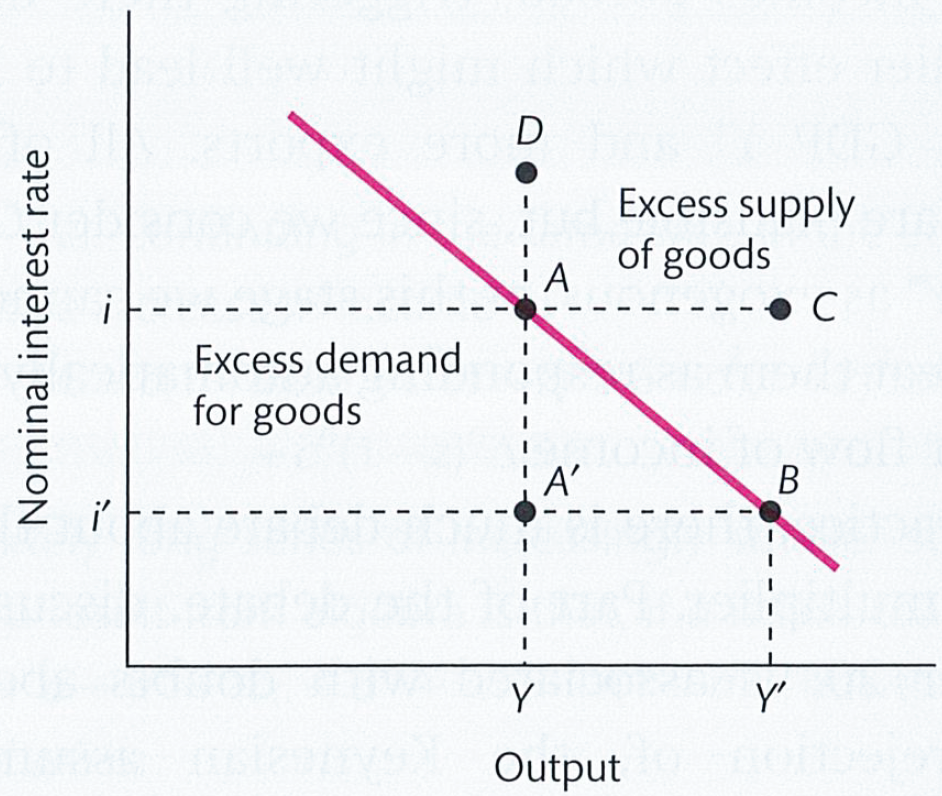
\includegraphics[trim=0 0 0 0,clip,width=0.5\textwidth]{FIGURES/6_IScurve}
	}      
	%\subfigure{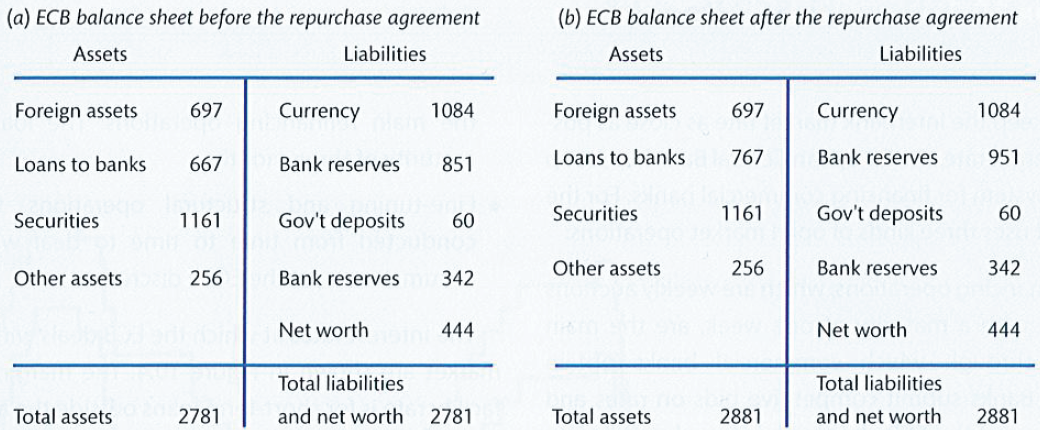
\includegraphics[trim=0 00 0 00,clip,width=0.6\textwidth]{FIGURES/5_CB_balance_sheet_OMO}
	%} 
	
%	\label{fig:GPD} 
	%[trim=left bottom right top
\end{figure}
%\vspace{-2mm}

\begin{minipage}{0.6\columnwidth}
\tiny	
%\textbf{Note.} Actual examples of trajectories, extracted from the French and Italian CPI databases. The dotted lines indicate events of price changes.
\textbf{Source.} Burda and Wyplosz (2017), Figure 11.3.\\
\end{minipage}
\end{center}
\end{frame}
%---FRAME------------------------------------------------------------------------------
\begin{frame}{The 45$^\circ$ graph and the IS curve}


\end{frame}

%%---FRAME------------------------------------------------------------------------------
%\begin{frame}{Shifts in the IS curve}
%
%\begin{itemize}
%\small
%\item Changes of \emph{endogenous} variables induce a \tb{movement along} the $IS$ curve ($Y$,$i$)
%\item Changes of \emph{exogenous} variables lead to a \tb{shift} of the $IS$ curve
%\item \emph{Example:} exogenous increase in aggregate demand ($G$)
%\item Multiplier effect: $A$ $\rightarrow$ $B$
%\item What shifts the $IS$ curve in practice? $G$, $T$, $\Omega$, $Y^*$, Tobin's $q$ (animal spirits)
%\end{itemize}
%
%\begin{center}
%%{\small
%%\tb{Figure.} Frequency of price increases and price decreases \\
%%}
%
%%\vspace{-2mm}
%\begin{figure}[h!]
%%\caption{Figure. Capital share US, 1946-2018
%	%\subfigure{\includegraphics<1>[trim=80 60 100 70,clip,width=0.75\textwidth]{FIGURES/3_Autarky}
%	%}
%	\subfigure{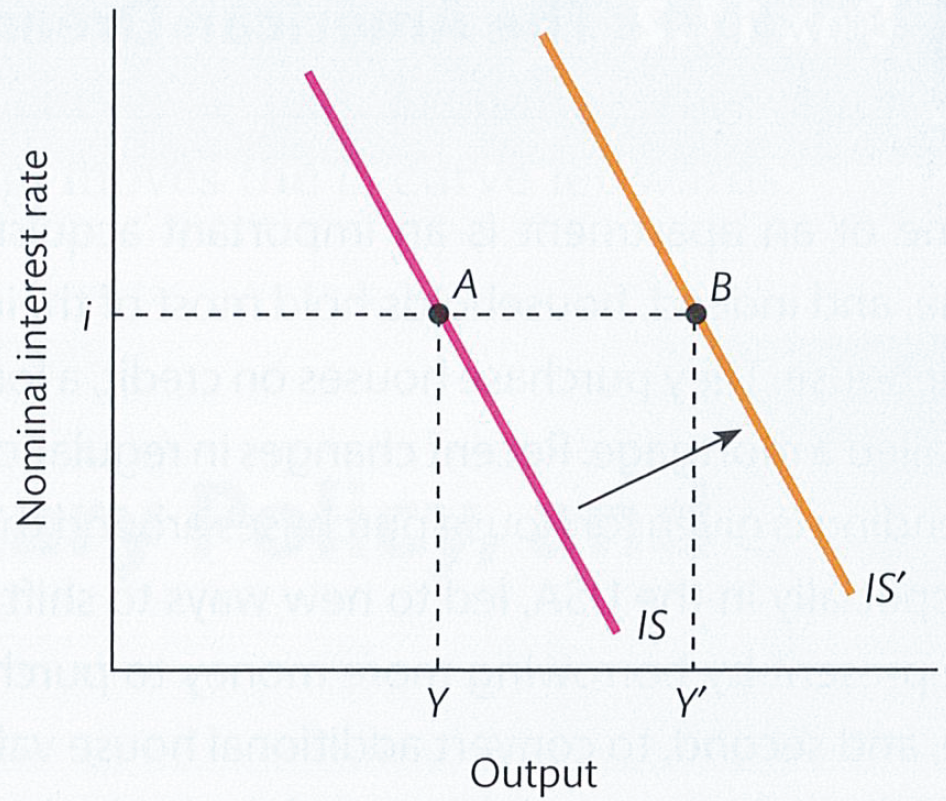
\includegraphics[trim=0 0 0 0,clip,width=0.5\textwidth]{FIGURES/6_IScurveShift}
%	}      
%	%\subfigure{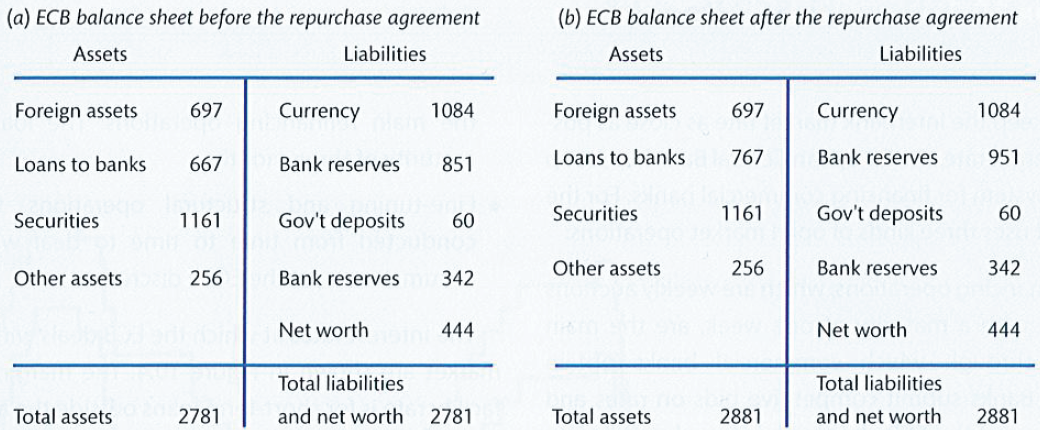
\includegraphics[trim=0 00 0 00,clip,width=0.6\textwidth]{FIGURES/5_CB_balance_sheet_OMO}
%	%} 
%	
%%	\label{fig:GPD} 
%	%[trim=left bottom right top
%\end{figure}
%%\vspace{-2mm}
%
%\begin{minipage}{0.6\columnwidth}
%\tiny	
%%\textbf{Note.} Actual examples of trajectories, extracted from the French and Italian CPI databases. The dotted lines indicate events of price changes.
%\textbf{Source.} Burda and Wyplosz (2017), Figure 11.4.\\
%\end{minipage}
%\end{center}
%
%\end{frame}
%---FRAME------------------------------------------------------------------------------
%---FRAME------------------------------------------------------------------------------
\begin{frame}{Moving along IS vs. shifting IS}
    \begin{columns}
\column{0.45\textwidth}
Changes in $i$ and resulting changes of $Y$ -- \textbf{movement along} IS \\
\vspace{0.5cm}
Change of any other determinant of DD -- \textbf{shift} of IS 
\vspace{0.5cm}
\column{0.55\textwidth}
\end{columns}
\end{frame}

\subsection{The Money Market, Monetary Policy and the TR Curve}
\begin{frame}
\tableofcontents[currentsubsection]{}
\end{frame}
%---FRAME------------------------------------------------------------------------------
\begin{frame}{Taylor rule and the TR curve}

Nominal interest rates are endogenous in the model. \\
\vfill
Nominal interest rates are set by the central bank as a function of the \tb{inflation gap} and the \tb{output gap} (\tm{Taylor rule}):
\begin{align*}
i = \bar{i} + a(\pi - \bar{\pi})+ b\left(\frac{Y-\bar{Y}}{\bar{Y}} \right)
\end{align*}
\vfill
Where $\bar Y$ is \tb{target output} of the central bank and $\bar \pi$ its \tb{target inflation}. \\
Assuming for now that inflation is always at its target:
\begin{align*}
i = \bar{i} + b\left(\frac{Y-\bar{Y}}{\bar{Y}} \right)
\end{align*}
Coefficient $\beta$ measures how \tb{active} the policy is
\end{frame}
\begin{frame}{Trend, cycle, and central bank's target GDP}
    \begin{columns}
\column{0.45\textwidth}
GDP data can be decomposed in \tb{trend} and \tb{cycles}: $Y^{actual} = Y^{trend} + Y^{cycle}$\\
\vspace{0.5cm}
Assumption: GDP would always be on smooth trend if prices were \textbf{flexible} \\
\vspace{0.5cm}
The goal of central bank is to \textbf{smoothen the cycles}, i.e. get closer to the trend GDP: $\bar Y = Y^{trend}$ 
\column{0.55\textwidth}
\end{columns}
\end{frame}
%---FRAME------------------------------------------------------------------------------
\begin{frame}{TR curve}

Taylor Rule (TR) equation is $i = \bar i + b \left(\frac{Y - \bar Y}{\bar Y}\right)$
\begin{itemize}
\item its graph in $(i, Y)$ space is an upward-sloping line
\item When $Y = \bar Y$, i.e. economy on trend, central bank sets $i = \bar{i}$ : the \tb{natural interest rate}
\item the economy is always on the TR curve as long as the central bank follows the Taylor Rule
\end{itemize}

\begin{center}
%{\small
%\tb{Figure.} Frequency of price increases and price decreases \\
%}

%\vspace{-2mm}
\begin{figure}[h!]
%\caption{Figure. Capital share US, 1946-2018
	%\subfigure{\includegraphics<1>[trim=80 60 100 70,clip,width=0.75\textwidth]{FIGURES/3_Autarky}
	%}
	\subfigure{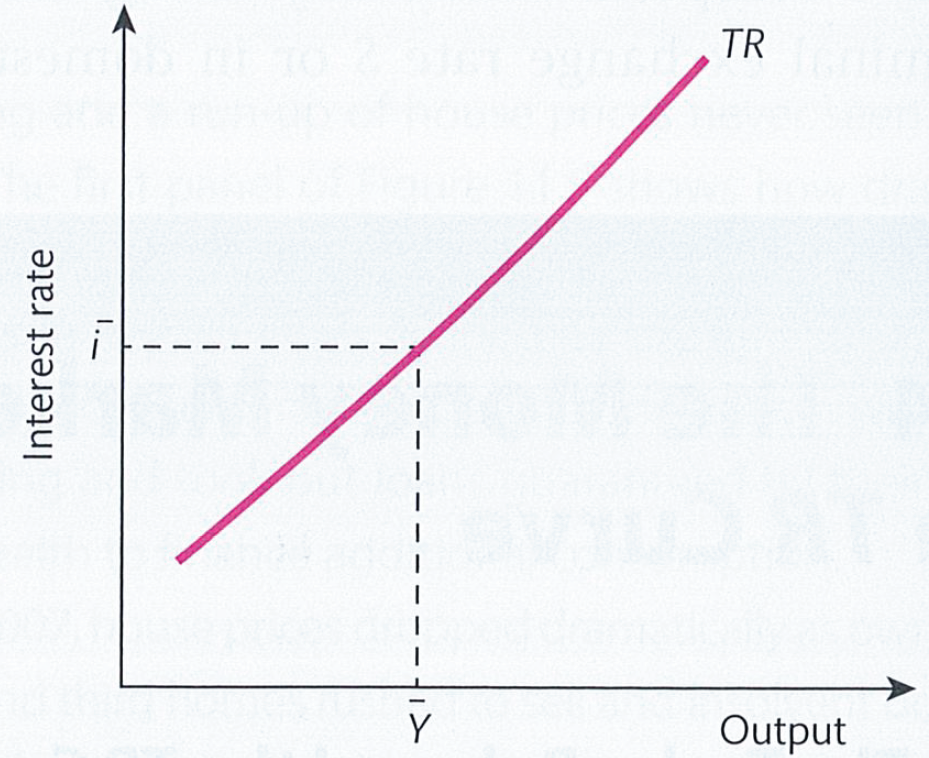
\includegraphics[trim=0 0 0 0,clip,width=0.4\textwidth]{FIGURES/6_TRcurve}
	}      
	%\subfigure{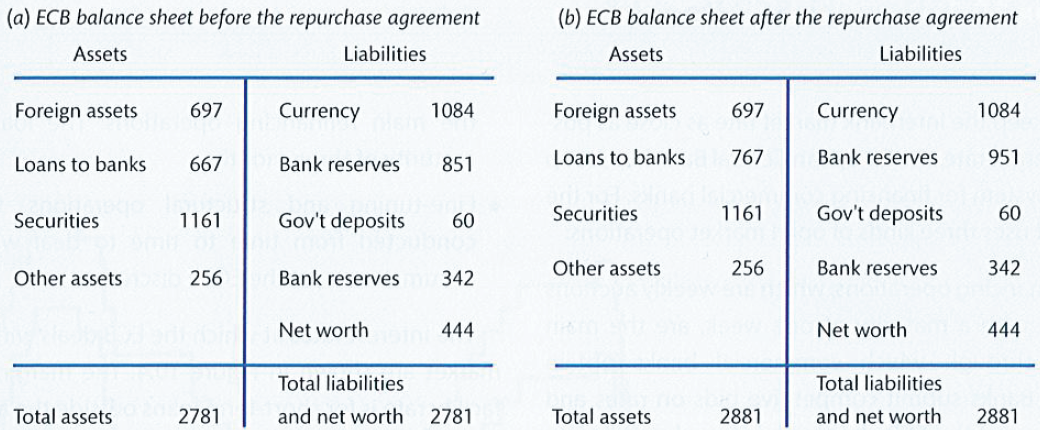
\includegraphics[trim=0 00 0 00,clip,width=0.6\textwidth]{FIGURES/5_CB_balance_sheet_OMO}
	%} 
	
%	\label{fig:GPD} 
	%[trim=left bottom right top
\end{figure}
%\vspace{-2mm}

\begin{minipage}{0.6\columnwidth}
\tiny	
%\textbf{Note.} Actual examples of trajectories, extracted from the French and Italian CPI databases. The dotted lines indicate events of price changes.
\textbf{Source.} Burda and Wyplosz (2017), Figure 11.6.\\
\end{minipage}
\end{center}

\end{frame}
%---FRAME------------------------------------------------------------------------------
%---FRAME------------------------------------------------------------------------------
%---FRAME------------------------------------------------------------------------------
%---FRAME------------------------------------------------------------------------------
\begin{frame}{Alternative assumption: Targeting Money Supply (LM)}
\begin{mytemize}
  \item During the 1980s, monetary targeting as main policy tool (M. Friedman)
\item Gives rise to the \tb{LM curve} (right graph) (\rarr IS-LM model  of J.R. Hicks)
\item %\tb{Money market equilibrium}: point $A$. A rise in output leads to higher money demand $M^{d'}$ (point $B$). 
  LM curve  upward sloping: pairs $(Y, i)$ for fixed supply of money $M^S$% \textcolor{red}{(same as case of Taylor Rule $TR_2$ above)}.
\end{mytemize}
\begin{center}
\begin{figure}[h!]
	\subfigure{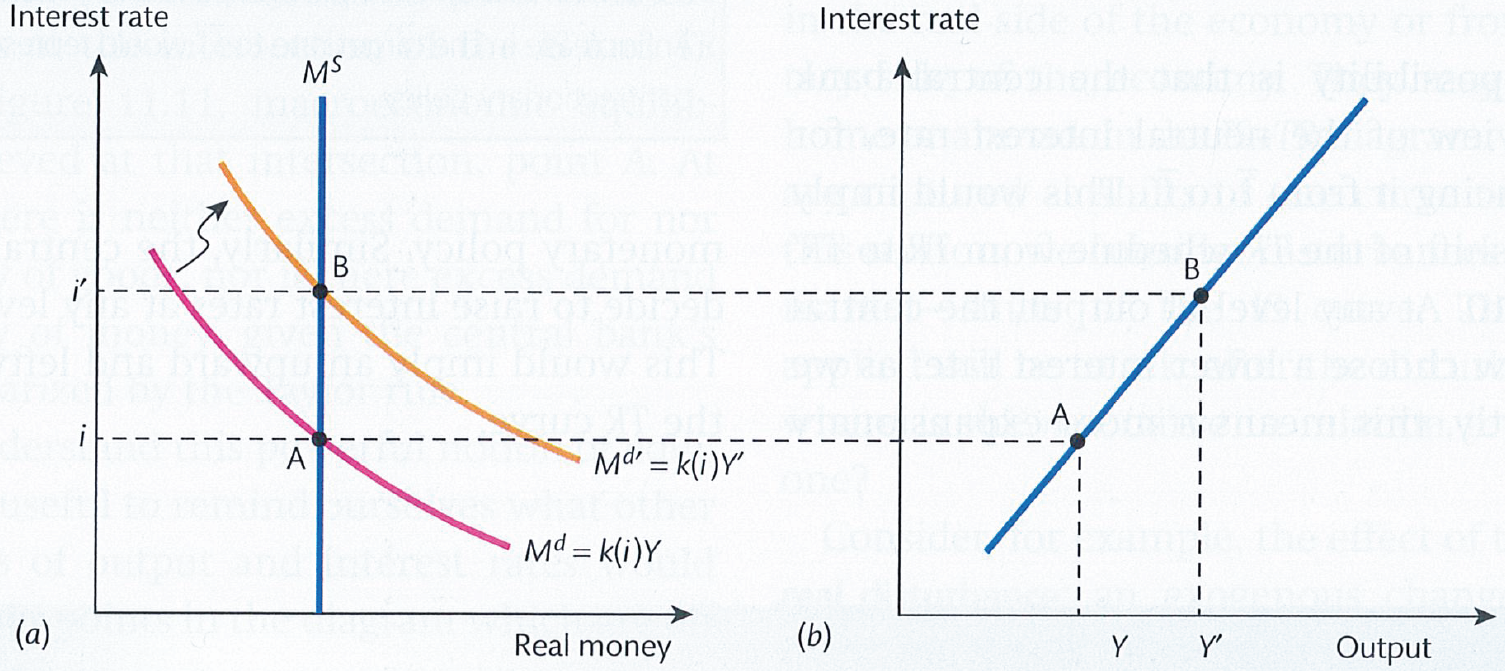
\includegraphics[trim=0 0 0 0,clip,width=0.95\textwidth]{FIGURES/6_LMcurve}
	}      
\end{figure}
\begin{minipage}{1.0\columnwidth}
\tiny	
\textbf{Note.} Panel (a) denotes the money market, the vertical $M^S$ line describes the central bank decision. Each money demand curve $M^d$ corresponds to a level of output. Panel (b) 
\textbf{Source.} Burda and Wyplosz (2017), Figure 11.9.\\
\end{minipage}
\end{center}
\end{frame}

\begin{frame}{Money market equilibrium with the TR curve}

\begin{itemize}
\item Expansion in GDP leads to higher interest rates (panel a) and higher demand for real money balances $(M/P)'$ (panel b).
\item \tb{Money market equilibrium} implies that the central bank provides this additional money in the form of reserves, which is consistent with $i$ given by the Taylor rule \alert{$(M^S)$}.
\end{itemize}

\begin{center}
%{\small
%\tb{Figure.} Frequency of price increases and price decreases \\
%}

%\vspace{-2mm}
\begin{figure}[h!]
%\caption{Figure. Capital share US, 1946-2018
	%\subfigure{\includegraphics<1>[trim=80 60 100 70,clip,width=0.75\textwidth]{FIGURES/3_Autarky}
	%}
	\subfigure{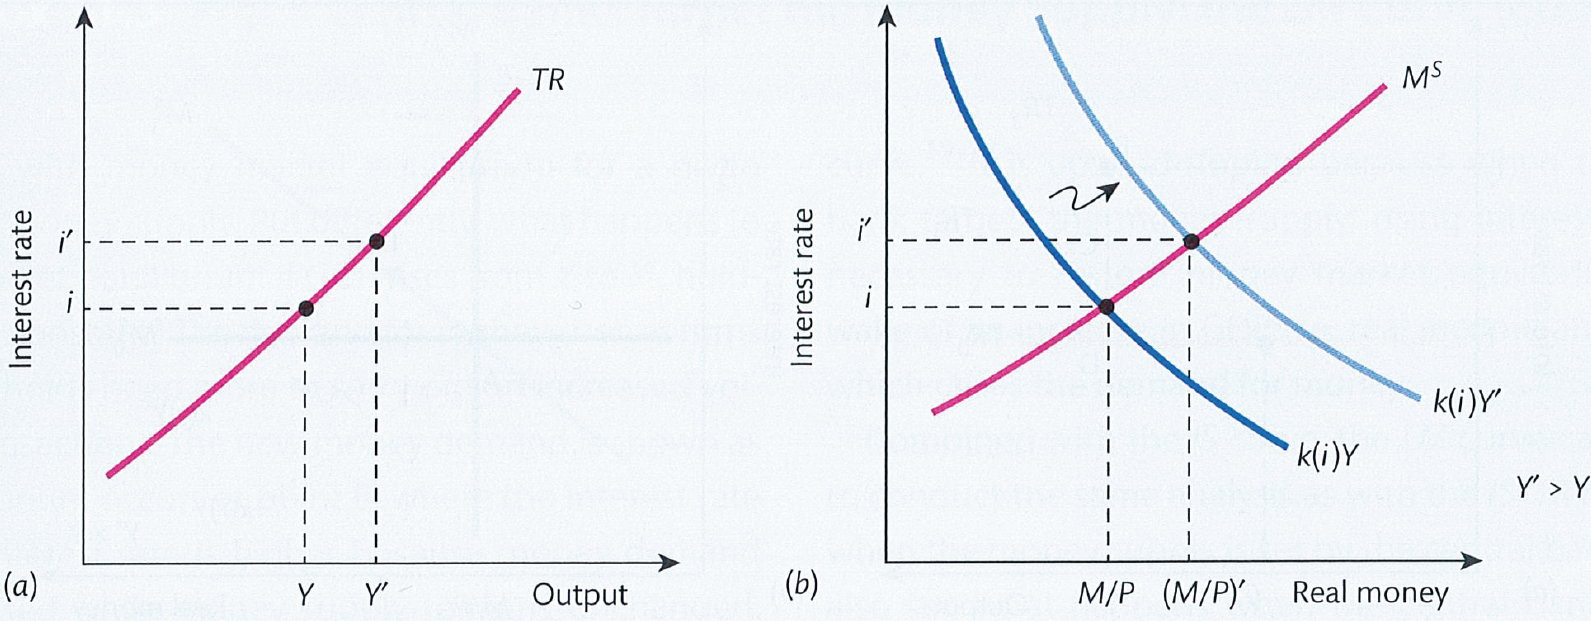
\includegraphics[trim=0 0 0 0,clip,width=0.9\textwidth]{FIGURES/6_MMequilibrium}
	}      
	%\subfigure{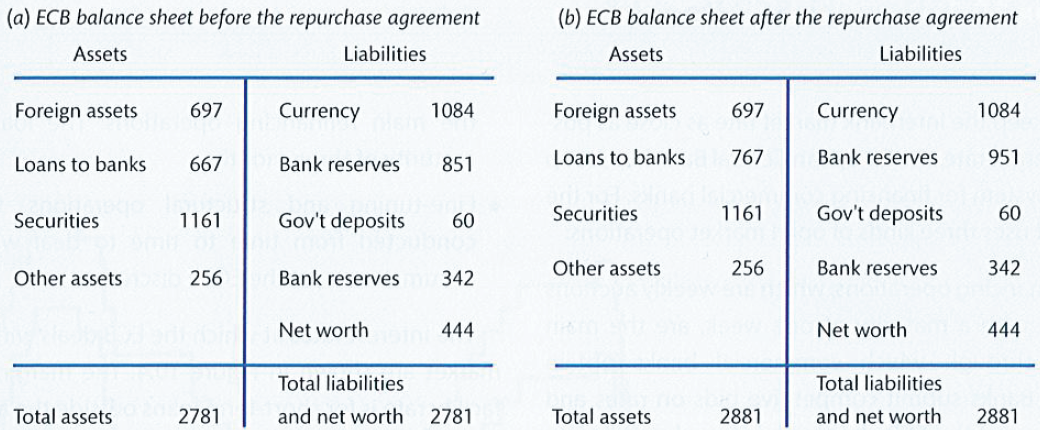
\includegraphics[trim=0 00 0 00,clip,width=0.6\textwidth]{FIGURES/5_CB_balance_sheet_OMO}
	%} 
	
%	\label{fig:GPD} 
	%[trim=left bottom right top
\end{figure}
%\vspace{-2mm}

\begin{minipage}{0.6\columnwidth}
\tiny	
%\textbf{Note.} Actual examples of trajectories, extracted from the French and Italian CPI databases. The dotted lines indicate events of price changes.
\textbf{Source.} Burda and Wyplosz (2017), Figure 11.7.\\
\end{minipage}
\end{center}

\end{frame}
%---FRAME------------------------------------------------------------------------------
%---FRAME------------------------------------------------------------------------------
%\begin{frame}{Slope of the TR curve}
%
%\begin{itemize}
%\small
%\item Reaction of nominal interest to output gap is related to reaction of money supply to 
%\item The coefficient $b$ in the Taylor rule captures the response.
%\begin{itemize}
%\small
%\item $TR_0$: perfectly elastic money money supply%($b=0$)
%\item $TR_1$: standard case
%\item $TR_2$: fixed money supply case
%\end{itemize}
%\end{itemize}
%
%\begin{center}
%%{\small
%%\tb{Figure.} Frequency of price increases and price decreases \\
%%}
%
%%\vspace{-2mm}
%\begin{figure}[h!]
%%\caption{Figure. Capital share US, 1946-2018
%	%\subfigure{\includegraphics<1>[trim=80 60 100 70,clip,width=0.75\textwidth]{FIGURES/3_Autarky}
%	%}
%	\subfigure{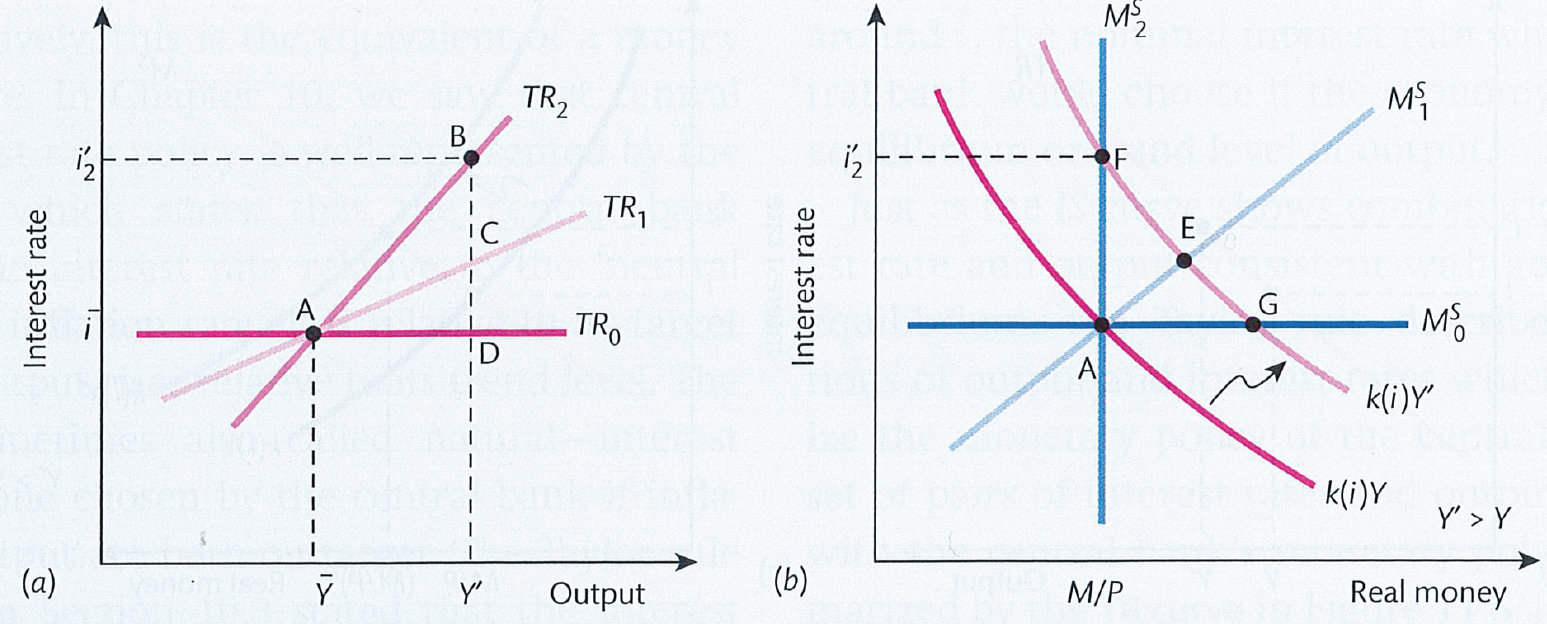
\includegraphics[trim=0 0 0 0,clip,width=0.95\textwidth]{FIGURES/6_TRcurveSlope}
%	}      
%	%\subfigure{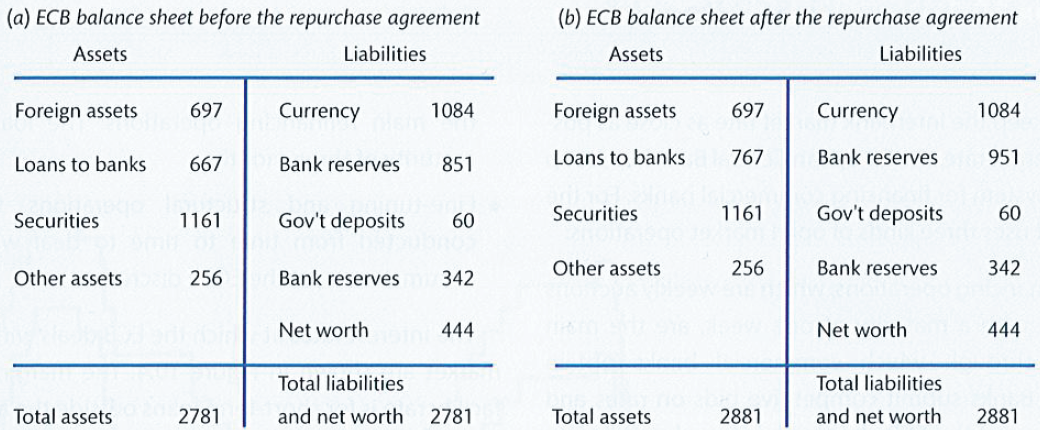
\includegraphics[trim=0 00 0 00,clip,width=0.6\textwidth]{FIGURES/5_CB_balance_sheet_OMO}
%	%} 
%	
%%	\label{fig:GPD} 
%	%[trim=left bottom right top
%\end{figure}
%%\vspace{-2mm}
%
%\begin{minipage}{0.6\columnwidth}
%\tiny	
%%\textbf{Note.} Actual examples of trajectories, extracted from the French and Italian CPI databases. The dotted lines indicate events of price changes.
%\textbf{Source.} Burda and Wyplosz (2017), Figure 11.8.\\
%\end{minipage}
%\end{center}
%
%\end{frame}
%---FRAME------------------------------------------------------------------------------
%---FRAME------------------------------------------------------------------------------
%---FRAME------------------------------------------------------------------------------
\begin{frame}{Movement along vs. shift of TR}


\begin{columns}
    \column{0.5\textwidth} For the simplified Taylor rule $i = \bar{i} + b\left(Y-\bar{Y}\right)/\bar{Y}$: \\ 
    \vspace{0.5cm}
    Changes in output \& the response of $i$ according to Taylor Rule \rarr \textbf{movement along} the TR line \\
    \vspace{0.5cm}
    A more active policy (larger $b$) means a more \textbf{steep} TR line \\
    \vspace{0.5cm}
    Change in the natural interest rate $\bar i$ \rarr \textbf{shift} of the TR line
    \column{0.5\textwidth}
\end{columns}


\end{frame}
%---FRAME------------------------------------------------------------------------------
\subsection{Macroeconomic Equilibrium}
%---FRAME------------------------------------------------------------------------------
\begin{frame}{Macroeconomic equilibrium in the IS-TR model}

We first study equilibrium in an economy where $TB=0$ constantly \textcolor{mint}{(does it mean the economy is closed?)} \\
\vfill
Definition of equilibrium: a pair of values $(Y, i)$ such that:
\begin{mynumerate}
\item   The goods market is in equilibrium (IS holds). This means $Y = DD$  
\item The Taylor Rule holds. This means the money market is also in equilibrium
\end{mynumerate}
\vfill
Geometrically, the point on the $(Y, i)$ plane where IS and TR lines intersect.
\end{frame}
%---FRAME------------------------------------------------------------------------------
\begin{frame}{Goods market shocks: shifts of IS}

Classic example: a shock of $G$. Note that $i$ changes in new equilibrium -- what are the implications for new equilibrium?

\begin{center}
%{\small
%\tb{Figure.} Frequency of price increases and price decreases \\
%}

%\vspace{-2mm}
\begin{figure}[h!]
%\caption{Figure. Capital share US, 1946-2018
	%\subfigure{\includegraphics<1>[trim=80 60 100 70,clip,width=0.75\textwidth]{FIGURES/3_Autarky}
	%}
	\subfigure{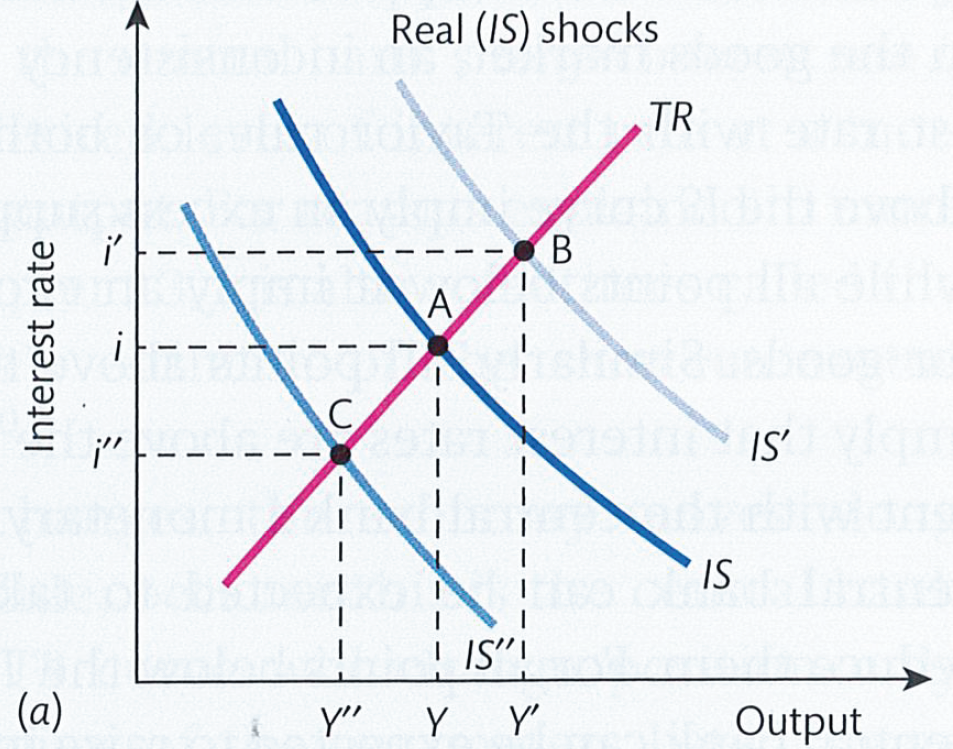
\includegraphics[trim=0 0 0 0,clip,width=0.6\textwidth]{FIGURES/6_ISTRadjustments_IS}
	}      
	%\subfigure{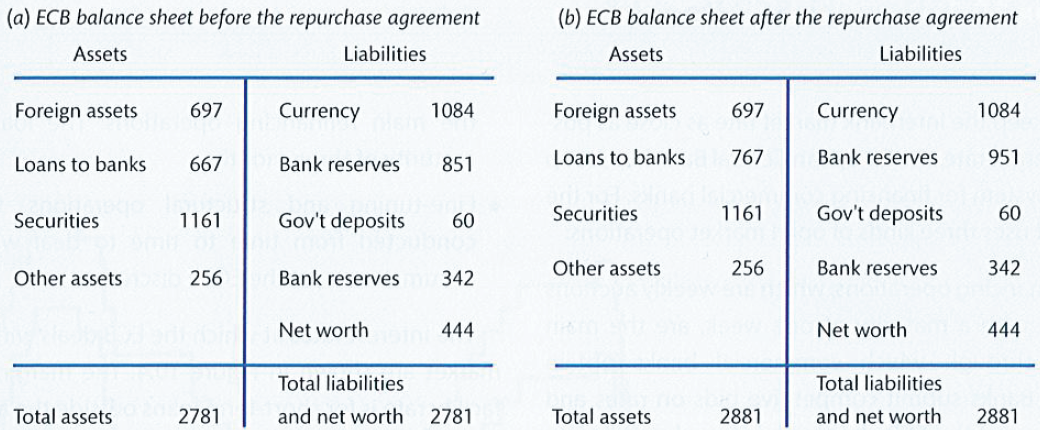
\includegraphics[trim=0 00 0 00,clip,width=0.6\textwidth]{FIGURES/5_CB_balance_sheet_OMO}
	%} 
	
%	\label{fig:GPD} 
	%[trim=left bottom right top
\end{figure}
%\vspace{-2mm}

\begin{minipage}{0.6\columnwidth}
\tiny	
%\textbf{Note.} Actual examples of trajectories, extracted from the French and Italian CPI databases. The dotted lines indicate events of price changes.
\textbf{Source.} Burda and Wyplosz (2017), Figure 11.12.\\
\end{minipage}
\end{center}
\vfill
Consider $G\uparrow$ \rarr IS shifts to the right. Central Bank responds \rarr $i \uparrow$. In the new equilibrium (point B), $C\uparrow$ and $G\uparrow$, but $I\downarrow$. Total effect on output is positive: $Y' > Y$.   
\end{frame}
%---FRAME------------------------------------------------------------------------------
\begin{frame}{Goods market shocks: mechanisms}

  Additional details on the ``shock propagation'':
\begin{mytemize}
\item How far does IS shift? Depends on the Keynesian multiplier
\item Other sources of goods market shocks:
\begin{mytemize}
\small
\item lump-sum taxes $T$ -- effect opposite to $G$, with a different multiplier \textcolor{mint}{(can you calculate it?)}
\item household wealth $\Omega$ -- same effect as $G$, multiplier depends on form of $C(\cdot)$
\item Tobin's q -- same effect as $G$
%\item the real exchange rate $\bar{\sigma}$
%\item foreign income $Y^*$
\end{mytemize}
\item Rest of the world shocks considered next week (remember, $TB=0$ assumed for now)
\end{mytemize}

\end{frame}
%---FRAME------------------------------------------------------------------------------
%---FRAME------------------------------------------------------------------------------
\begin{frame}{Monetary policy shocks}

Assume the Central Bank revises its $\bar i$ (which can happen because the natural interest rate is not measured directly): 
  
\begin{center}

\begin{figure}[h!]
	\subfigure{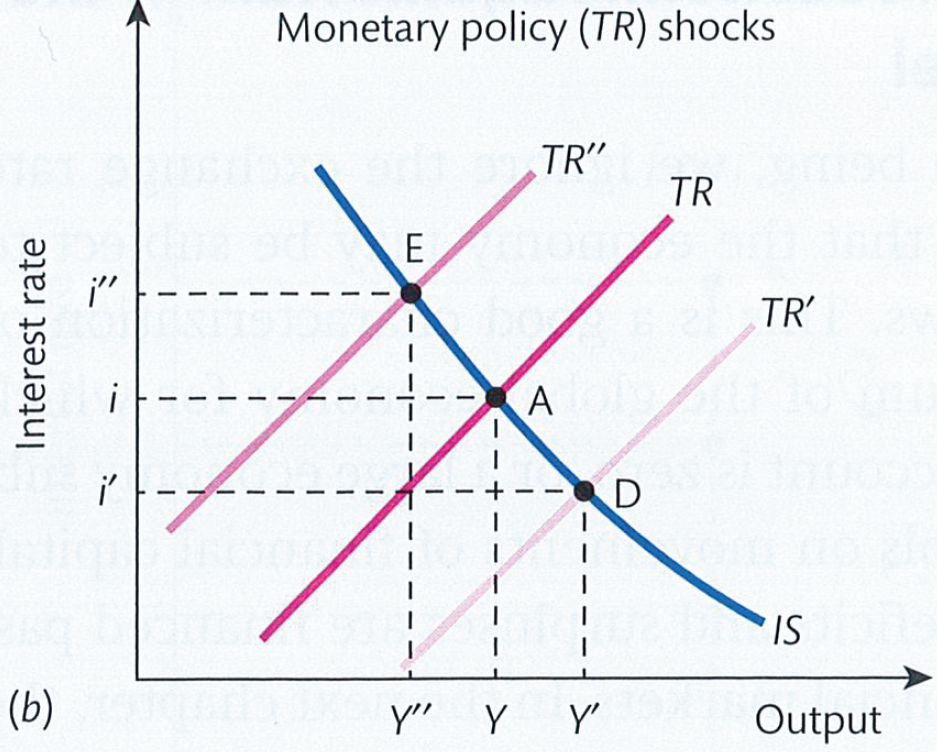
\includegraphics[trim=0 0 0 0,clip,width=0.6\textwidth]{FIGURES/6_ISTRadjustments_TR}
	}      
\end{figure}

\begin{minipage}{0.6\columnwidth}
\tiny	
\textbf{Source.} Burda and Wyplosz (2017), Figure 11.12 (b).\\
\end{minipage}
\end{center}

Consider $\bar i \downarrow$ \rarr 
 TR shifts down
  \rarr $r\downarrow$, $I \uparrow$, $Y\uparrow$ \rarr  \tb{expansionary} monetary policy

\end{frame}

%---FRAME------------------------------------------------------------------------------
\begin{frame}{How to use the IS-TR framework}

Be able to answer two main questions:
\begin{mynumerate}
\item Which line (IS or TR) is affected by shock(s)?
\item In what direction do IS and TR move?
\item Find new equilibrium geometrically, then think about mechanisms -- the always involve $i$ and $I$
\end{mynumerate}
Shocks tend to happen simultaneously:
\begin{mytemize}
\item A boost in public spending and a tax raise
\item A fall in natural rate of the Central Bank and a rise in investors' optimism
\end{mytemize}
\vfill
In the first case, the joint effect on both $Y$ and $i$ is ambiguous, in the second $Y\uparrow$, but the final change in $i$ unclear \textcolor{mint}{(verify that)}

\end{frame}
%---FRAME------------------------------------------------------------------------------
\begin{frame}{A linear closed economy model}
  
\textbf{Consumption function}
\begin{align*}
C = & a_0 + a_1 \Omega + b(Y-T) \\
= & a+b(Y-T), 
\end{align*}
where $a=a_0 + a_1 \Omega$ is the autonomous part of $C$ (does not depend on income), and $b < 1$ is the \tb{mpc}
\vfill
\textbf{Investment function}
\begin{align*}
I = c + dY +ei,
\end{align*}
with $c, d > 0$, \textcolor{red}{$e < 0$} \\
\vfill
\textbf{Simplified Taylor rule}
\begin{align*}
  i = \bar i + \beta(Y- \bar Y)
\end{align*}
Output gap not normalized by $\bar Y$\\
\vfill
\tm{Solve for the macro equilibrium before first TD}
%
%\tb{Exports}
%\begin{align*}
%X = x_0 + x_1Y^* -x_2 \sigma
%\end{align*}
%
%\tb{Imports}
%\begin{align*}
%Z=z_0+z_1 Y + z_2 \sigma
%\end{align*}
%
%Combining exports and imports yields the \tb{primary current account fct} as
%\begin{align*}
%PCA &= f - gY +g^* Y^* -h \sigma,
%\end{align*}
%where $f=x_0-z_0$, $g=z_1$, $g^*=x_1$, and $h=x_2+z_2$.



\end{frame}
%---FRAME------------------------------------------------------------------------------
%---FRAME------------------------------------------------------------------------------
%---FRAME------------------------------------------------------------------------------
%---FRAME------------------------------------------------------------------------------
%---FRAME------------------------------------------------------------------------------
%---FRAME------------------------------------------------------------------------------
%\begin{frame}{The zero lower bound in the IS-TR model}
%
%\begin{center}
%%{\small
%%\tb{Figure.} Frequency of price increases and price decreases \\
%%}
%
%%\vspace{-2mm}
%\begin{figure}[h!]
%%\caption{Figure. Capital share US, 1946-2018
%	%\subfigure{\includegraphics<1>[trim=80 60 100 70,clip,width=0.75\textwidth]{FIGURES/3_Autarky}
%	%}
%	\subfigure{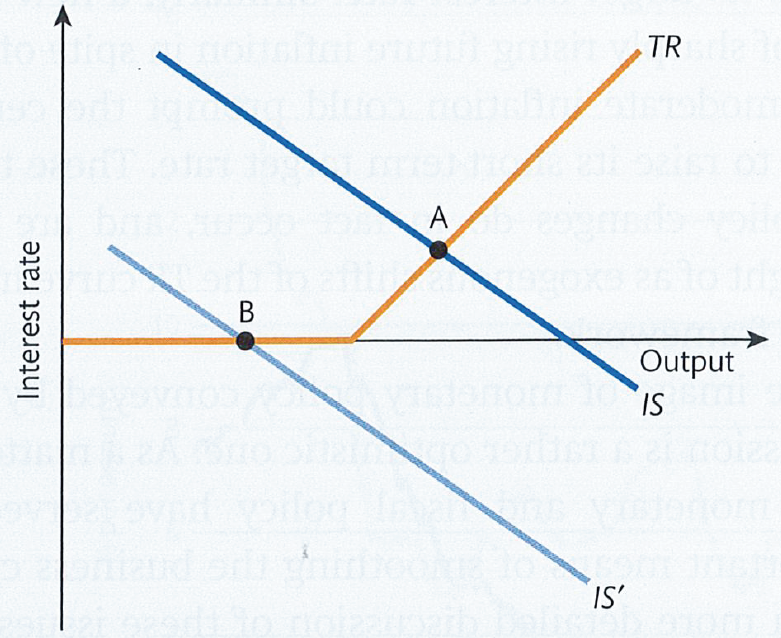
\includegraphics[trim=0 0 0 0,clip,width=0.45\textwidth]{FIGURES/6_ISTRmodelZLB}
%	}      
%	%\subfigure{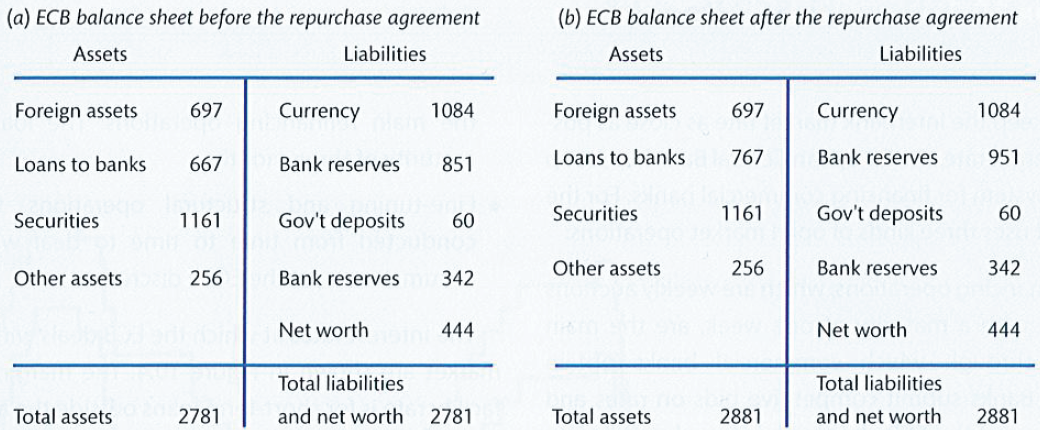
\includegraphics[trim=0 00 0 00,clip,width=0.6\textwidth]{FIGURES/5_CB_balance_sheet_OMO}
%	%} 
%	
%%	\label{fig:GPD} 
%	%[trim=left bottom right top
%\end{figure}
%%\vspace{-2mm}
%
%\begin{minipage}{0.6\columnwidth}
%\tiny	
%%\textbf{Note.} Actual examples of trajectories, extracted from the French and Italian CPI databases. The dotted lines indicate events of price changes.
%\textbf{Source.} Burda and Wyplosz (2017), Figure 11.14.\\
%\end{minipage}
%\end{center}
%
%\end{frame}
%---FRAME------------------------------------------------------------------------------
%---FRAME------------------------------------------------------------------------------
%---FRAME------------------------------------------------------------------------------
%---FRAME------------------------------------------------------------------------------
%---FRAME------------------------------------------------------------------------------
%---FRAME------------------------------------------------------------------------------
%---FRAME------------------------------------------------------------------------------
%---FRAME------------------------------------------------------------------------------

\begin{frame}{Summary: IS-TR}


\begin{itemize}
\item We studied a \tb{demand-driven} equilibrium with \tb{fixed prices}
\item A Keynesian \tb{Multiplier} measures how much the GDP consistent with goods market equilibrium changes after shock
\item \tb{IS} curve: GDP levels and interest rates compatible with equilibrium in the goods market
\item \tb{TR} curve: central bank setting of $i$ to smoothen business cycles
\item Macroeconomic equilibrium in an economy with $TB=0$ intersection $IS$ and $TR$
\end{itemize}

\end{frame}

%%---FRAME------------------------------------------------------------------------------
%---END------------------------------------------------------------------------------
%\begin{frame}
%
%\vspace{10mm}
%\begin{center}
%{\Large
%\tb{Thank you.}\\
%}
%\vspace{10mm}
%\footnotesize{
%{\color{dblue}{\texttt{christoph.grossesteffen@banque-france.fr}}
%}}
%\end{center}
%
%\end{frame}
%---END------------------------------------------------------------------------------
\end{document}

